\chapter{Neutron - Gamma Discrimination}
\label{chap:SecElectron}

Effective neutron-gamma discrimination is integral to the performance of the detector.
Generally, two methods are available for discrimination; 1) pulse shape discrimination and 2) pulse height discrimination.
In pulse shape discrimination the different decay times between the neutron and gamma pulses are exploited to develop a metric that allows for the classification of the pulse.
Generally, pulse shape discrimination works best when the pulses are noticeably different.
Pulse height discrimination is based on setting a pulse height discriminator that acts as a partition between two classes of pulses.
This is generally easier to implement than pulse shape discrimination.
While some of the fabricated films show a small basis for pulse shape discrimination, this work will only focus on pulse height discrimination.

The pulse height discriminator setting necessary to achieve the neutron-gamma discrimination is achieved through the use of a mathematical lower level discriminator (MLLD).
This virtual discriminator establishes the bound where $\epsilon_{int,\gamma n}\leq 10^{-6}$, and counts above the MLLD are classified as neutron counts. 

It is currently understood that the light output per path length of the film (which is directly proportional to the pulses collected on the PMT) is related to the stopping power of the radiation in the film material.
This is described by the Birks equation \eqref{eqn:BirksEquation}
\begin{align}
  \label{eqn:BirksEquation}
  \frac{dL}{dx} = \frac{S_B\frac{dE}{dx}}{1+kB\frac{dE}{dx}}
\end{align}
where \definevar{$S_B$}{absolute scintillation efficiency},\definevar{$\frac{dE}{dx}$}{linear stopping power} and \definevar{$kB$}{Birks parameter}.
For a given material the stopping power of the film will be constant, and therefore the light output of the film can be found by integrating the light output per path length over the total length of the film.
It is then possible to observe that the light output of a film is proportional to the energy deposited in the film.

Preferential energy deposition by neutrons relative to gammas will enhance the discrimination by creating larger neutron light pulses than the gamma pulses, allowing for fewer neutron pulses to be classified as gamma pulses because they are below the MLLD.
Thus, neutron-gamma discrimination can be enhanced by optimizing the energy deposition in the film. 

The organization of this chapter is as follows.
An overview of scintillation mechanics of organic scintillators will be provided in \autoref{sec:ScintMechanics} in order to understand the relationship between scintillation and the energy deposited by charged particles.
The energy spectra and ranges of neutron and gamma reaction products will be discussed in \autoref{sec:InteractionsAndRange} (focusing on polystyrene) to explain the basis for the difference in energy depositions. 
Calculations of the energy deposition will be shown in \autoref{sec:EnergyDep} for polymeric materials, providing the foundation of neutron-gamma pulse height discrimination.

%%%%%%%%%%%%%%%%%%%%%%%%%%%%%%%%%%%%%%%%%%%%%%%%%%%%%%%%%%%%%%%%%%%%%%%%%%%
%                                                                         %
%                      SCINTILLATION MECHANICS                            %
%                                                                         %
%%%%%%%%%%%%%%%%%%%%%%%%%%%%%%%%%%%%%%%%%%%%%%%%%%%%%%%%%%%%%%%%%%%%%%%%%%%
\section{Scintillation Mechanisms}
\label{sec:ScintMechanics}
%%%%%%%%%%%%%%%%%%%%%%%%%%%%%%%%%%%%%%%%%%%%%%%%%%%%%%%%%%%%%%%%%%%%%%%%%%%
%                                                                         %
%                         Introduction to Scintillation                   %
%                                                                         %
%%%%%%%%%%%%%%%%%%%%%%%%%%%%%%%%%%%%%%%%%%%%%%%%%%%%%%%%%%%%%%%%%%%%%%%%%%%
Scintillation detecctors (the detectors on which this work is based) utilize a scintillator to convert ionizing radiation into photons, and then transporting and capturing those the emitted photons, commonly with a photomultiplier tube (PMT).
The electrical signal from the PMT is then an indicator of a radiation event in the detector's scintillator material.
The current RPM's with \iso[3]{He} are ion chamber detectors, however, the proposed \iso[6]{Li} glass detectors and \iso[6]{LiF} doped ZnS:Ag detectors are scintillation based detectors. 

\subsection{Organic Scintillators}
An organic scintillator generally has a $\pi$-electron structure, as shown in \autoref{fig:pielectron}.
An incoming particle (generally electrons liberated from the energy deposition of the ionizing radiaiton) then excites one of the modes of the $\pi$-electron structure.
Higher singlet states rapidly (on the order of picoseconds) relax to the first singlet state, and excessive vibrational energy (populations of the vibrational sates) is lost.
Thus, after a short period of time the entire excitation population is in the $S_10$ state, and the decay of this state creates the prompt fluorescence.
\begin{figure}
  \centering
  \includegraphis[width=\textwidth]{PiElectronSates}
  \caption[$\pi$ Electron Structure]{Typicall $\pi$-electron structure of an organic molecule. The ground state of the molecule is shown as $S_0$, and excited single states are $S_1$, $S_2$ etc The triplet states are $T_1$, $T_2$, with the vibrational states as $S_OO$, $S_01$, $S_02$ and so forth. Figure from Wikipedia.}
  \label{fig:pielectron}
\end{figure}
The exictations of triplet states typically yield delayed scintillation events or phosphorescence.
An exicted triplet states immediately decays to the $T_0$ state by internal degration without a photon emission.
The $T_0$ state typically decays by interacting with another $T_0$ state in a $T_0 + T_0 \to S^* + S_0 + h\nu$ transition.
The excited singlet state $S^*$ then also decays to the $S_0$ state.
The $T_0 + T_0$ transitions is slower than direct singlet state dexcitations, and results in a slow component of the pulse, which can be used for pulse shape discrimination.

Several factors need to be considered in order of a material to be considred as a scintilaltor:
\begin{itemize}
  \item The light yield should be linearly proportional to the energy deposition
  \item The material should be optically transparent to it's own wavelength of emission
  \item A short rise time with a fast decay time
\end{itemize}
Scintillators convert the energy deposited in the material by ionizing radiation in to photons.



%%%%%%%%%%%%%%%%%%%%%%%%%%%%%%%%%%%%%%%%%%%%%%%%%%%%%%%%%%%%%%%%%%%%%%%%%%%
%                                                                         %
%                      ENERGY SCALE AND RANGES                            %
%                                                                         %
%%%%%%%%%%%%%%%%%%%%%%%%%%%%%%%%%%%%%%%%%%%%%%%%%%%%%%%%%%%%%%%%%%%%%%%%%%%
\section{Charged Particle Interactions and Ranges}
\label{sec:InteractionsAndRange}
%%%%%%%%%%%%%%%%%%%%%%%%%%%%%%%%%%%%%%%%%%%%%%%%%%%%%%%%%%%%%%%%%%%%%%%%%%%
%                                                                         %
%                      ENERGY SCALE AND RANGES                            %
%                                                                         %
%%%%%%%%%%%%%%%%%%%%%%%%%%%%%%%%%%%%%%%%%%%%%%%%%%%%%%%%%%%%%%%%%%%%%%%%%%%
The theoretical basis for the difference in energy deposition lies in the different mechanisms between charged particle interactions and photon interactions in matter.
For photons with energies between approximately \SI{0.5}{\MeV} and \SI{5}{\MeV} Compton scattering is the predominant interaction mechanism between the material and the photon.
The probability of an electron having a given kinetic energy after scattering can be expressed as \autoref{eqn:dSdEKlienNishina} (see \autoref{ch:ComptonScatter} for derivation details)
\begin{align}
  \label{eqn:dSdEKleinNishina}
\frac{d\sigma}{dE_e} = 2\pi r_e^2 \sin \theta f(\theta)\left [ \frac{1+\frac{E}{m_e c^2}\left(1-\cos\theta \right)^2}{E^2 \sin \theta} \right ]
\end{align}
provided  $f(\theta)$ is defined as $f(\theta) = \frac{1}{2}\left(\frac{E'}{E}\right)^2 \left(\frac{E'}{E} + \frac{E}{E'}-\sin^2\theta\right)$.
This distribution is shown for \iso[60]{Co} in \autoref{fig:Co60ComptonScatterSpectra}.
It is then highly likely that the Compton scattered electron will have an energy close to that of the maximum energy for the Compton scattering, \SI{0.96}{\MeV} for the \SI{1.173}{\MeV} photon and \SI{1.12}{\MeV} for the \SI{1.33}{\MeV} photon.
\begin{figure}
  \centering
  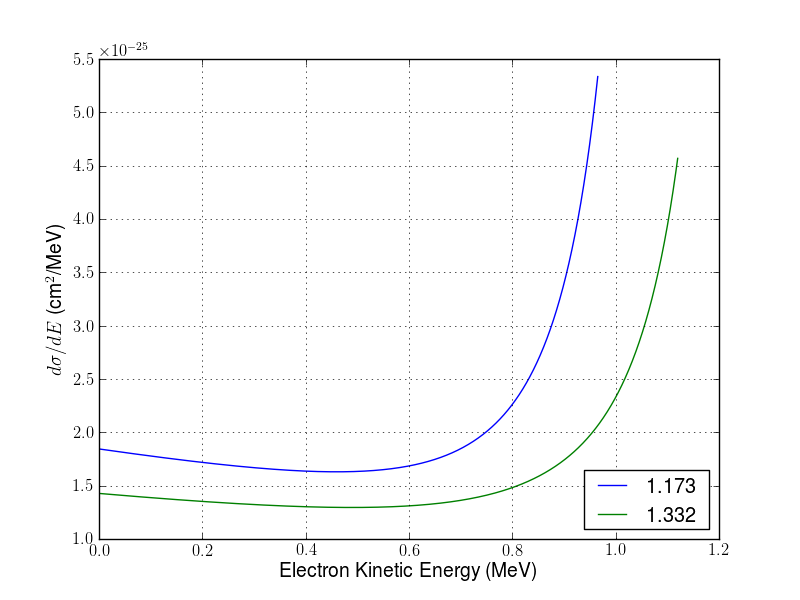
\includegraphics[width=\textwidth]{Co60ComptonScatteredSpectra}
  \caption[Gamma (Co-60) Compton Scattered Spectra]{Probability per energy of an Compton Scattered Electron having a given kinetic energy from \iso[60]{Co}}
  \label{fig:Co60ComptonScatterSpectra}
\end{figure}
The cumulative distribution function (CDF) is shown in \autoref{fig:Co60ComptonScatterCDF}.
\begin{figure}
  \centering
  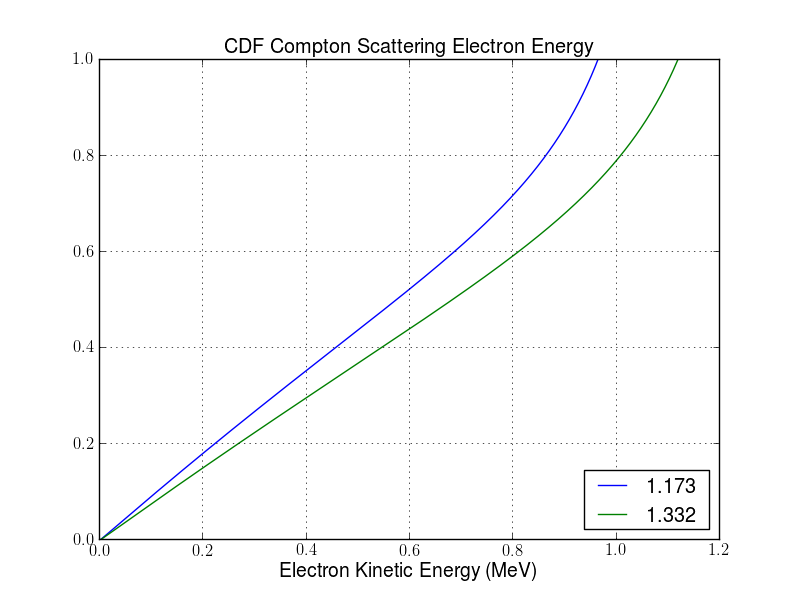
\includegraphics[width=\textwidth]{Co60ComptonScatteredSpectraCDF}
  \caption[Gamma (Co-60) Compton Scattered CDF]{Probability of the energy of a Compton Scattered Electron from \iso[60]{Co}. Over half of the electrons from the Compton scattering will have an energy greater than \SI{0.5}{\MeV}}
  \label{fig:Co60ComptonScatterCDF}
\end{figure}
In the case of $\iso[6]{Li}\left(n,\iso[3]{H}\right)\alpha$ the fission energy is distributed between a triton of energy \SI{2.73}{\mega\eV} and an alpha of energy \SI{2.05}{\mega\eV}.
The maximum kinetic energy of an electron from a Compton scattering event with an impingement \iso[60]{Co} source is \SI{1.117}{\mega\eV} (for the \SI{1.332}{\mega\eV} gamma). 
In polystyrene with a density of \SI{1}{\gram\per\cm\cubed}, the range of the maximum electron from Compton scattering is around \SI{4.5E3}{\um}\cite{berger_estar_2005}.
If elastic scattering between the alpha, triton and electrons is assumed the maximum kinetic energy of an electron is \SI{1.097}{\kilo\eV} for the alpha particle and \SI{1.986}{\kilo\eV} for the triton\cite{turner_atoms_2008}.
The range of the electron from a gamma interaction is more than \num{1E3} times greater than the range of electrons from an alpha or triton (Table \ref{tab:BasicEDepOutline}).
Therefore, it is more likely that the electrons generated by the alpha and the triton deposit significantly more of their energy in a thin film than the electron from a gamma.
This is also reflected in the stopping power, where the reaction product secondary electrons have a stopping power 40 times that of the secondary electrons from a gamma \cite{berger_estar_2005}.
The simulated electron range distributions for several energies is shown in \autoref{fig:ElectronRanges}.
\begin{table}[ht]
  \caption{Electron Energy, Range, and Stopping Power\protect\cite{berger_estar_2005,turner_atoms_2008}}
	\centering
	\begin{tabular}{c | c S c}
	{Electron Parent} & {Electron Energy} & {Total Stopping Power} & {CSDA Range} \\
	 &  & \si{\mega\eV \cm\squared \per \gram} & \si{\gram\per\cm\squared} \\
	\hline
	\hline
	{gamma}  & \SI{1.12}{\mega\eV} & 1.79 & $\ge$~\num{4.48E-1} \\
	{triton} & \SI{1.99}{\kilo\eV} & 75.1 & $\le$~\num{2.55E-4} \\
	{alpha}  & \SI{1.10}{\kilo\eV} & 113  & $\le$~\num{2.55E-4} \\
	\end{tabular}
  \label{tab:BasicEDepOutline}
	% See pg. 87 of Matthew's lab notebook for the calculation
\end{table}
\begin{figure}
  \centering
    \begin{subfigure}[b]{0.45\textwidth}
      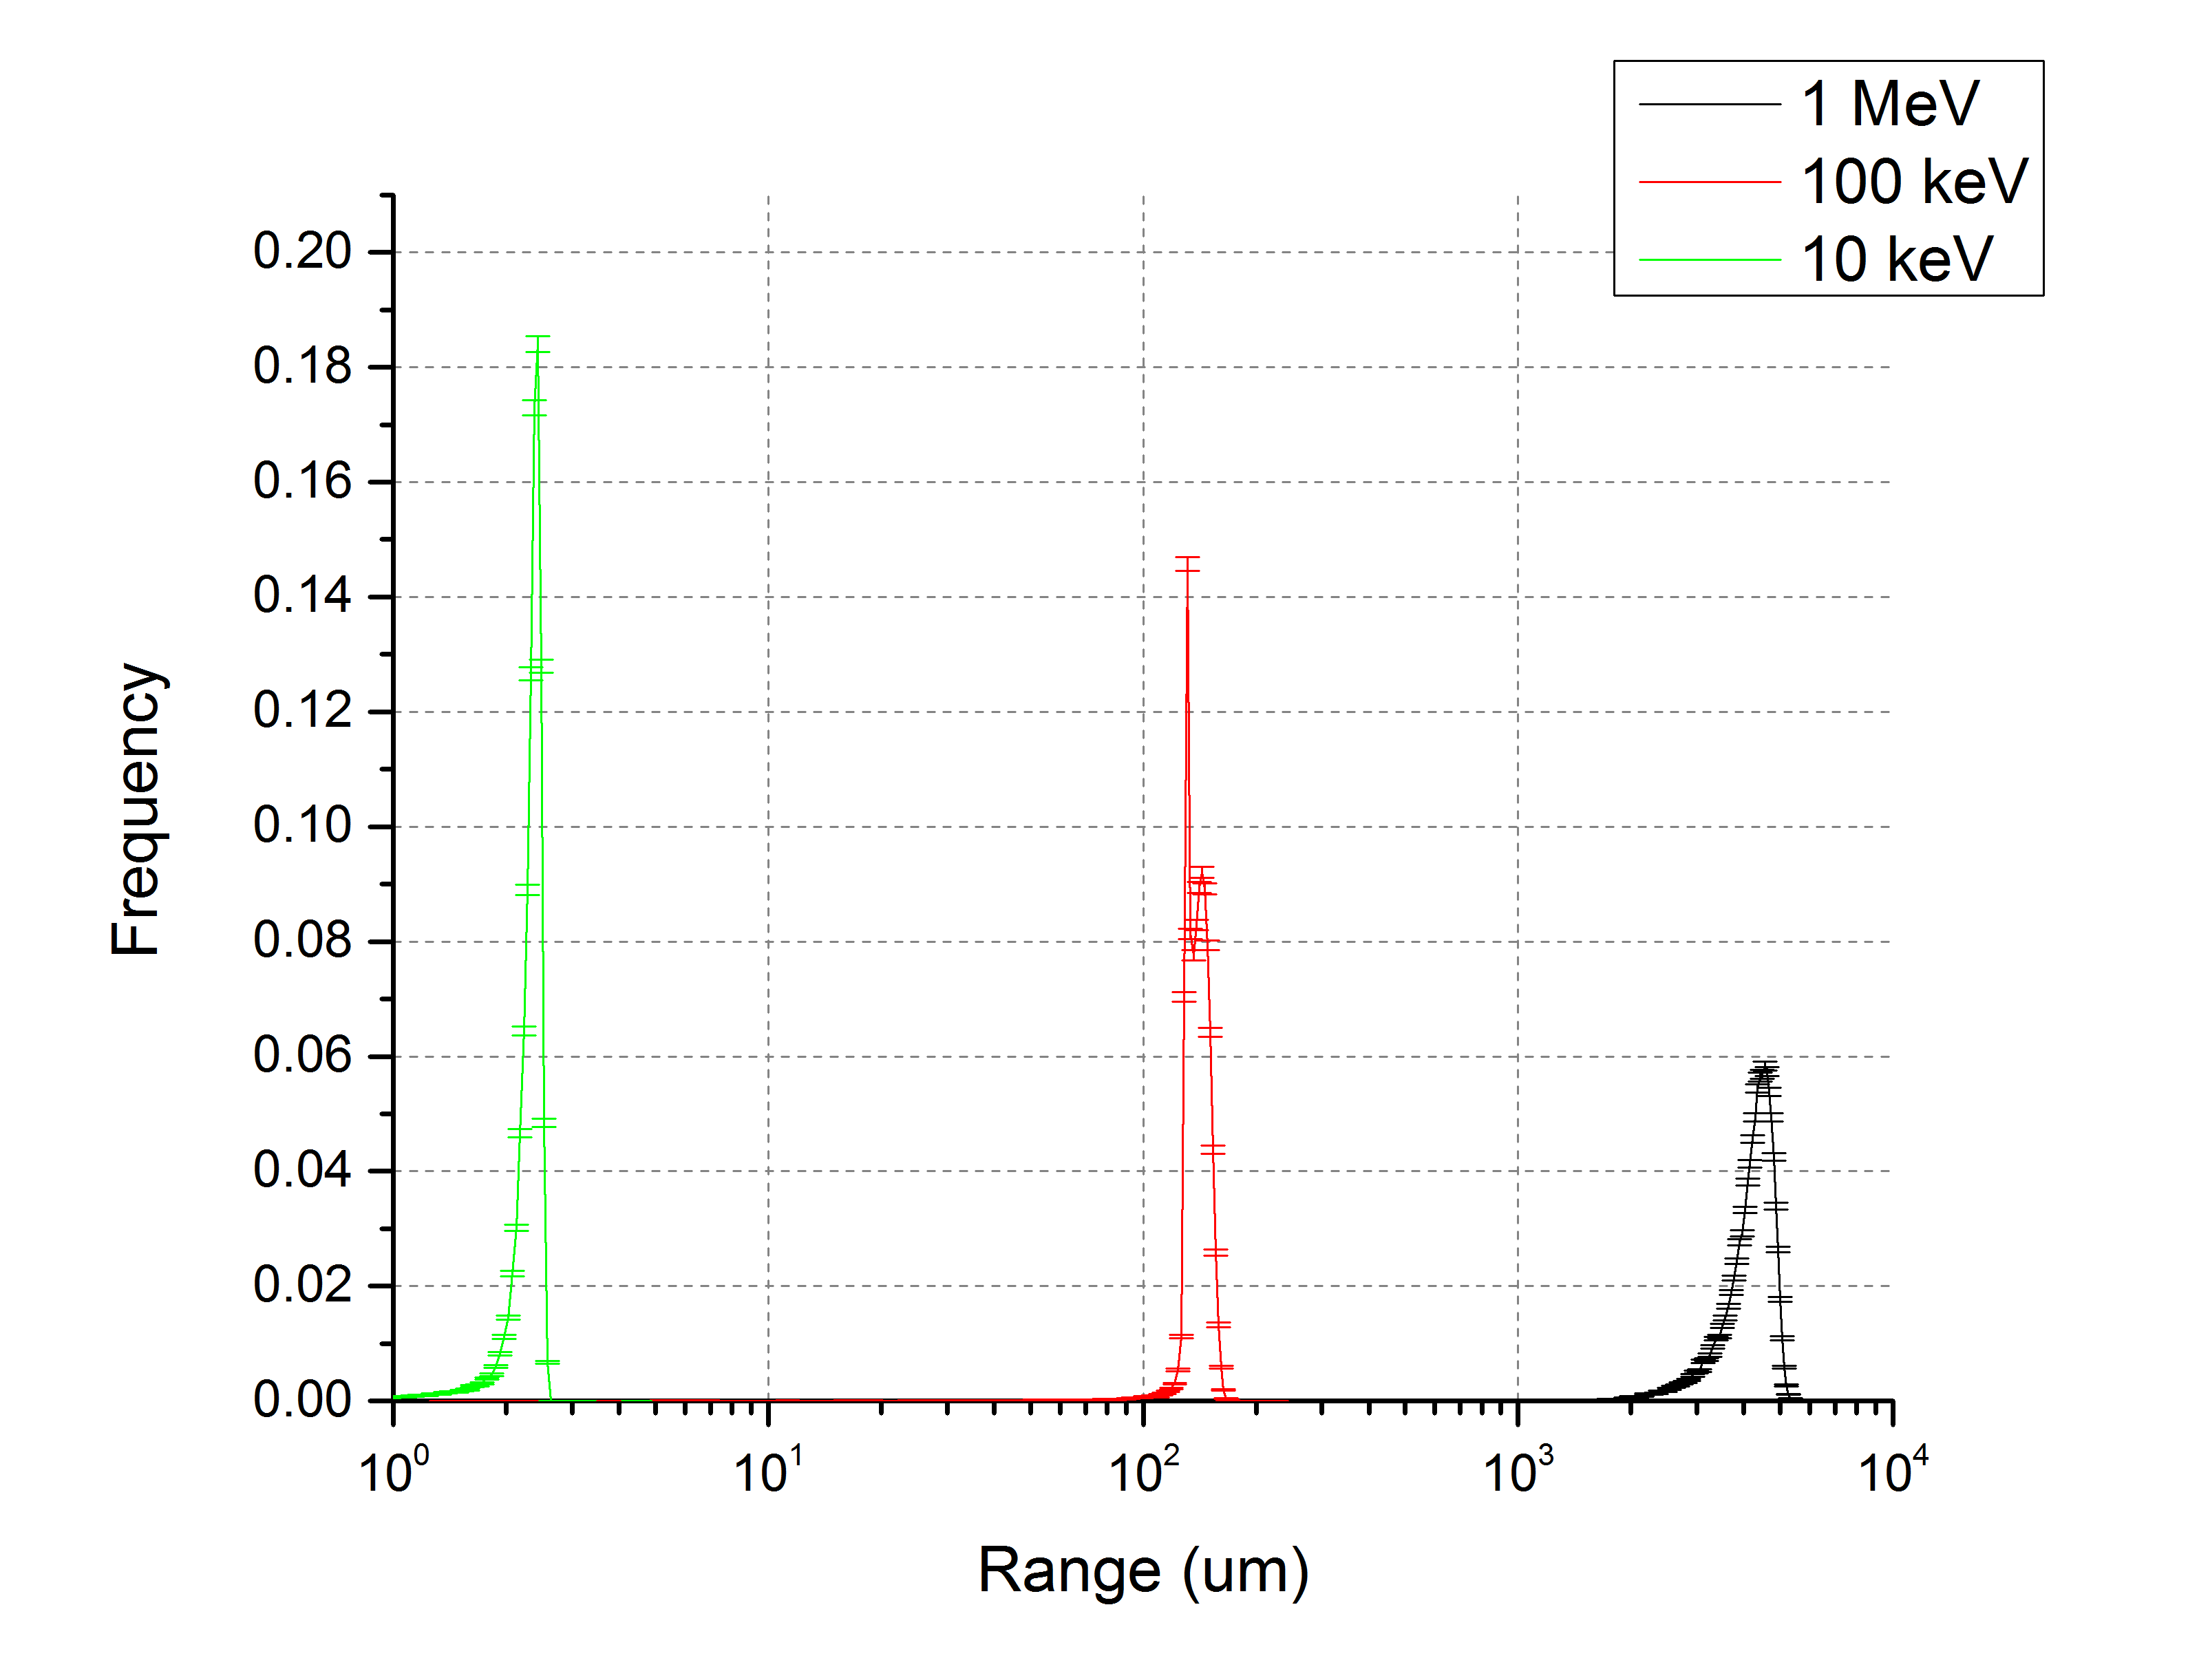
\includegraphics[width=\textwidth]{ElectronRangeDistribution}
      \caption[Range of \SI{1}{\MeV}, \SI{100}{\keV}, and \SI{10}{\keV} electrons]{Simulated ranges (GENAT4) of \SI{1}{\MeV}, \SI{100}{\keV}, and \SI{10}{\keV} electrons.}
    \end{subfigure}%
    ~
    \begin{subfigure}[b]{0.45\textwidth}
      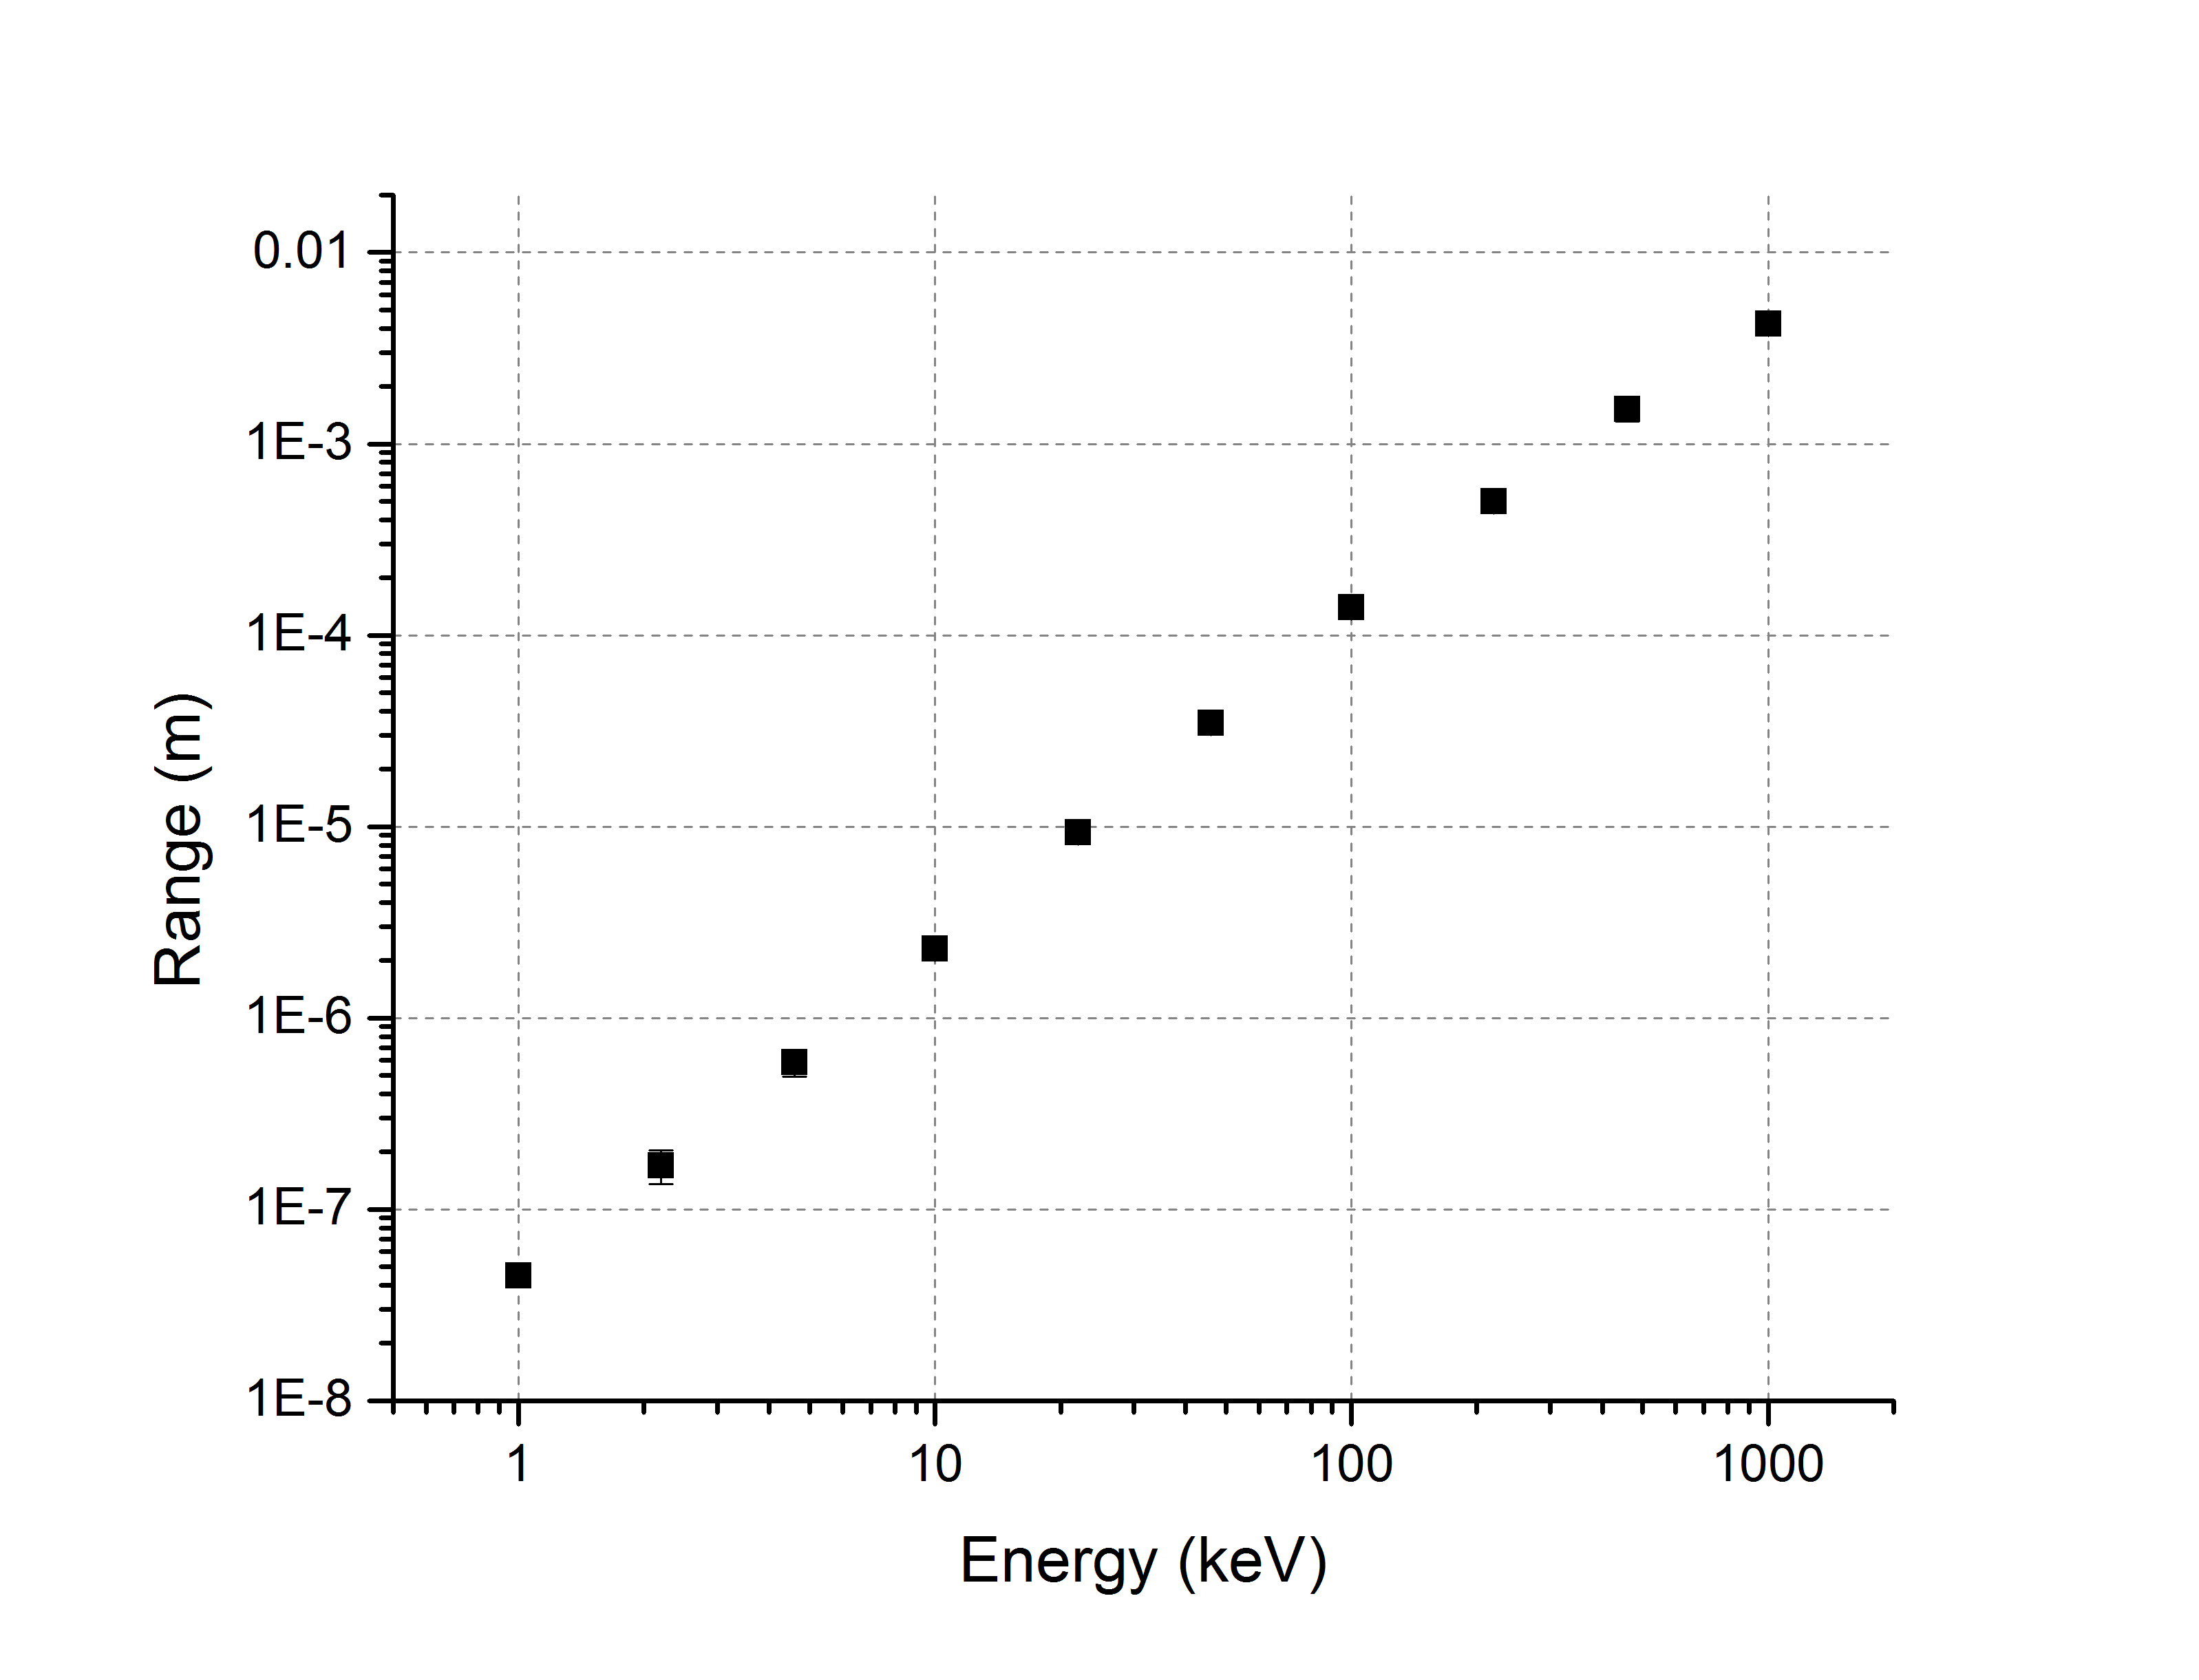
\includegraphics[width=\textwidth]{ElectronRange}
      \caption[Range of Electrons in Polystyrene]{Simulated (GEANT4) range of electrons in polystyrene. Compton scatted electrons from \iso[60]{Co} on the order of  \~ 100 keV will have ranges two orders of magnitude than that of electrons from the charged particle interactions.}
    \end{subfigure}
  \label{fig:ElectronRanges}
\end{figure}

The development of the secondary electron energy ranges so far has been from a simplified treatment of the problem when only the dominant process are considered.
Detailed simulations are necessary in order to have a greater understanding of the problem. 
The energy of the electrons created from an alpha (\SI{2.05}{\MeV}), triton (\SI{2.73}{\MeV}), and gammas from \iso[60]{Co} were calculated using a GEANT4 simulation, and overlaid on the range of electrons as shown in \autoref{fig:ERangeAndDist}.
It is then clear that the electrons from the \iso[60]{Co} will travel much father than those from the $\iso[6]{Li}\left(n,\alpha\right)\iso[3]{H}$ reaction products.
\begin{figure}
  \centering
  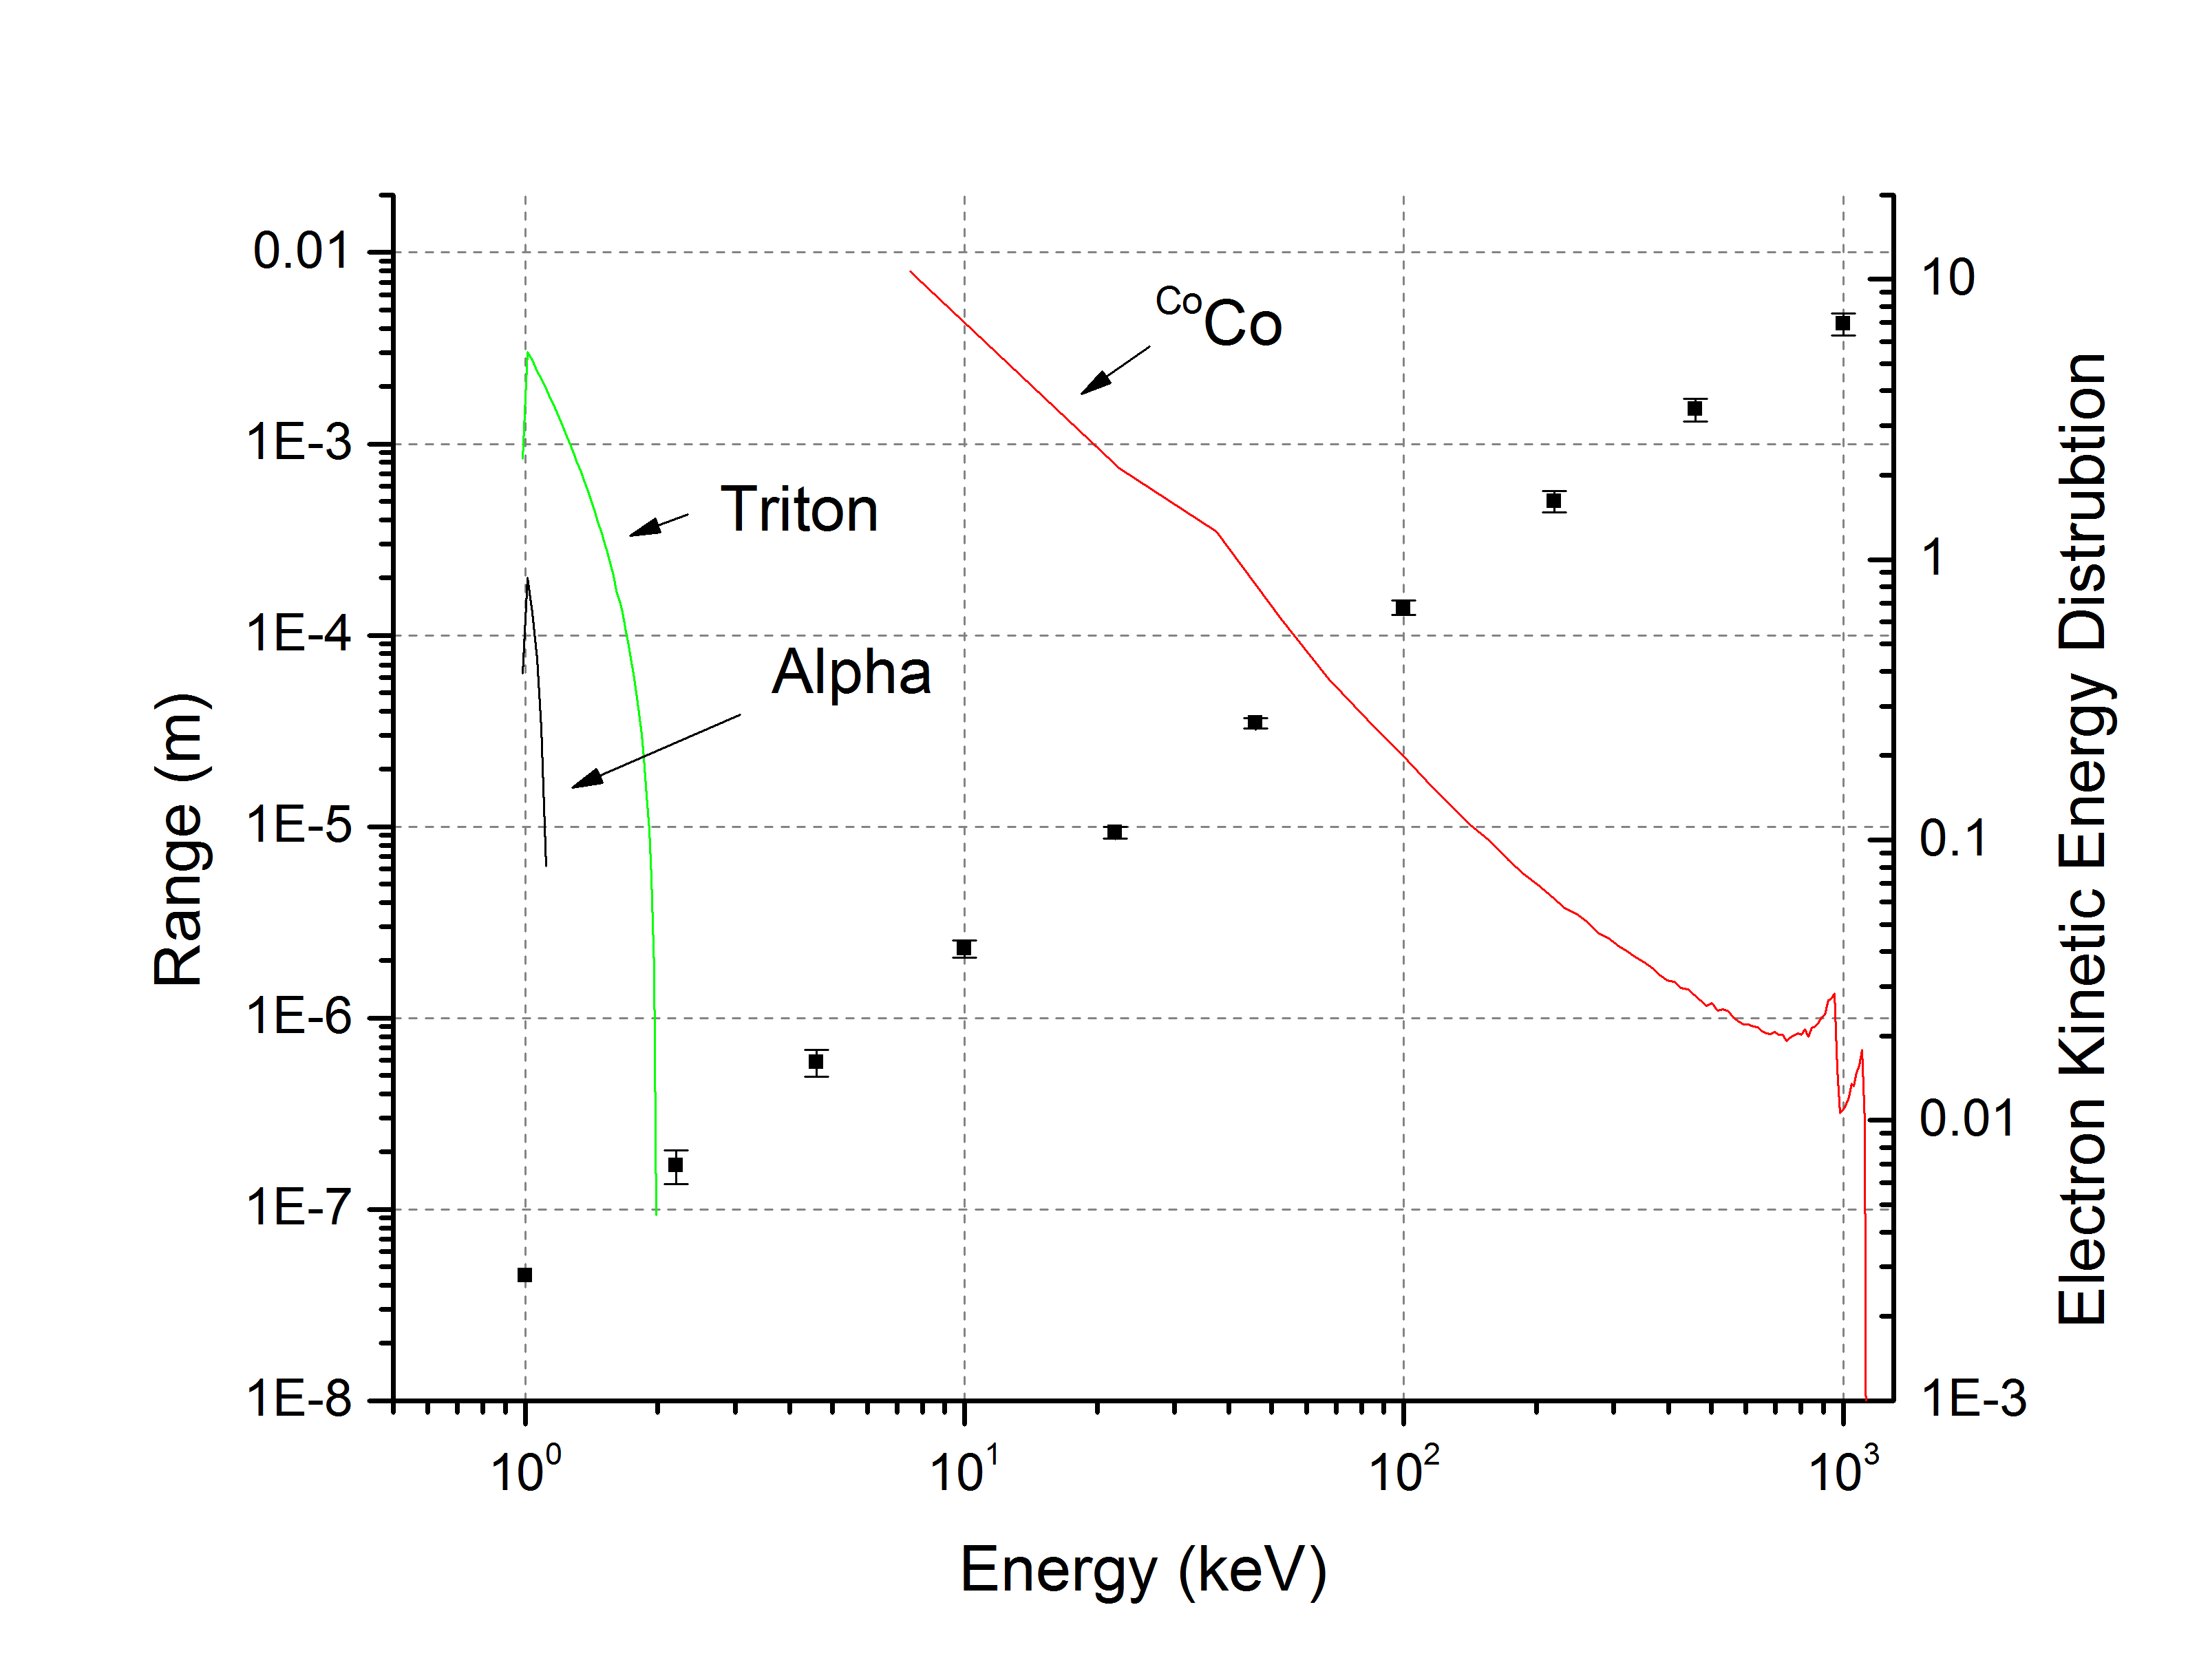
\includegraphics[width=\textwidth]{ElectronRangeAndEnergyDist}
  \caption[Electron Range and Energy Distribution of Selected Reactions]{The electron range (left axis) overlaid with the kinetic energy of electrons from \SI{2.05}{\MeV} alpha, \SI{2.73}{\MeV} triton, and gammas from \iso[60]{Co}. The \iso[60]{Co} electrons have energies much greater than the alpha and triton}
  \label{fig:ERangeAndDist}
\end{figure}

%%%%%%%%%%%%%%%%%%%%%%%%%%%%%%%%%%%%%%%%%%%%%%%%%%%%%%%%%%%%%%%%%%%%%%%%%%%
%                                                                         %
%                     ENERGY DEPOSITION SIMULATIONS                       %
%                                                                         %
%%%%%%%%%%%%%%%%%%%%%%%%%%%%%%%%%%%%%%%%%%%%%%%%%%%%%%%%%%%%%%%%%%%%%%%%%%%

\section{Energy Deposition Simulations}
\label{sec:EnergyDeposition}
The GEANT4 toolkit has the ability to track the energy deposition in different materials as well as the tracking of electrons to a least \SI{1}{\keV}\cite{agostinelli_geant4simulation_2003}.
It is proposed to represent the detector geometry as a single layer of neutron absorbing thin polymeric film mounted on top of a non-scintillating material (PMMA).
For simplicity, the initial events for runs will be chosen by setting up a particle gun for thermal (\SI{0.025}{\eV}) neutrons upon the detector and for both gammas resulting from a \iso[60]{Co} decay.
\begin{figure}
  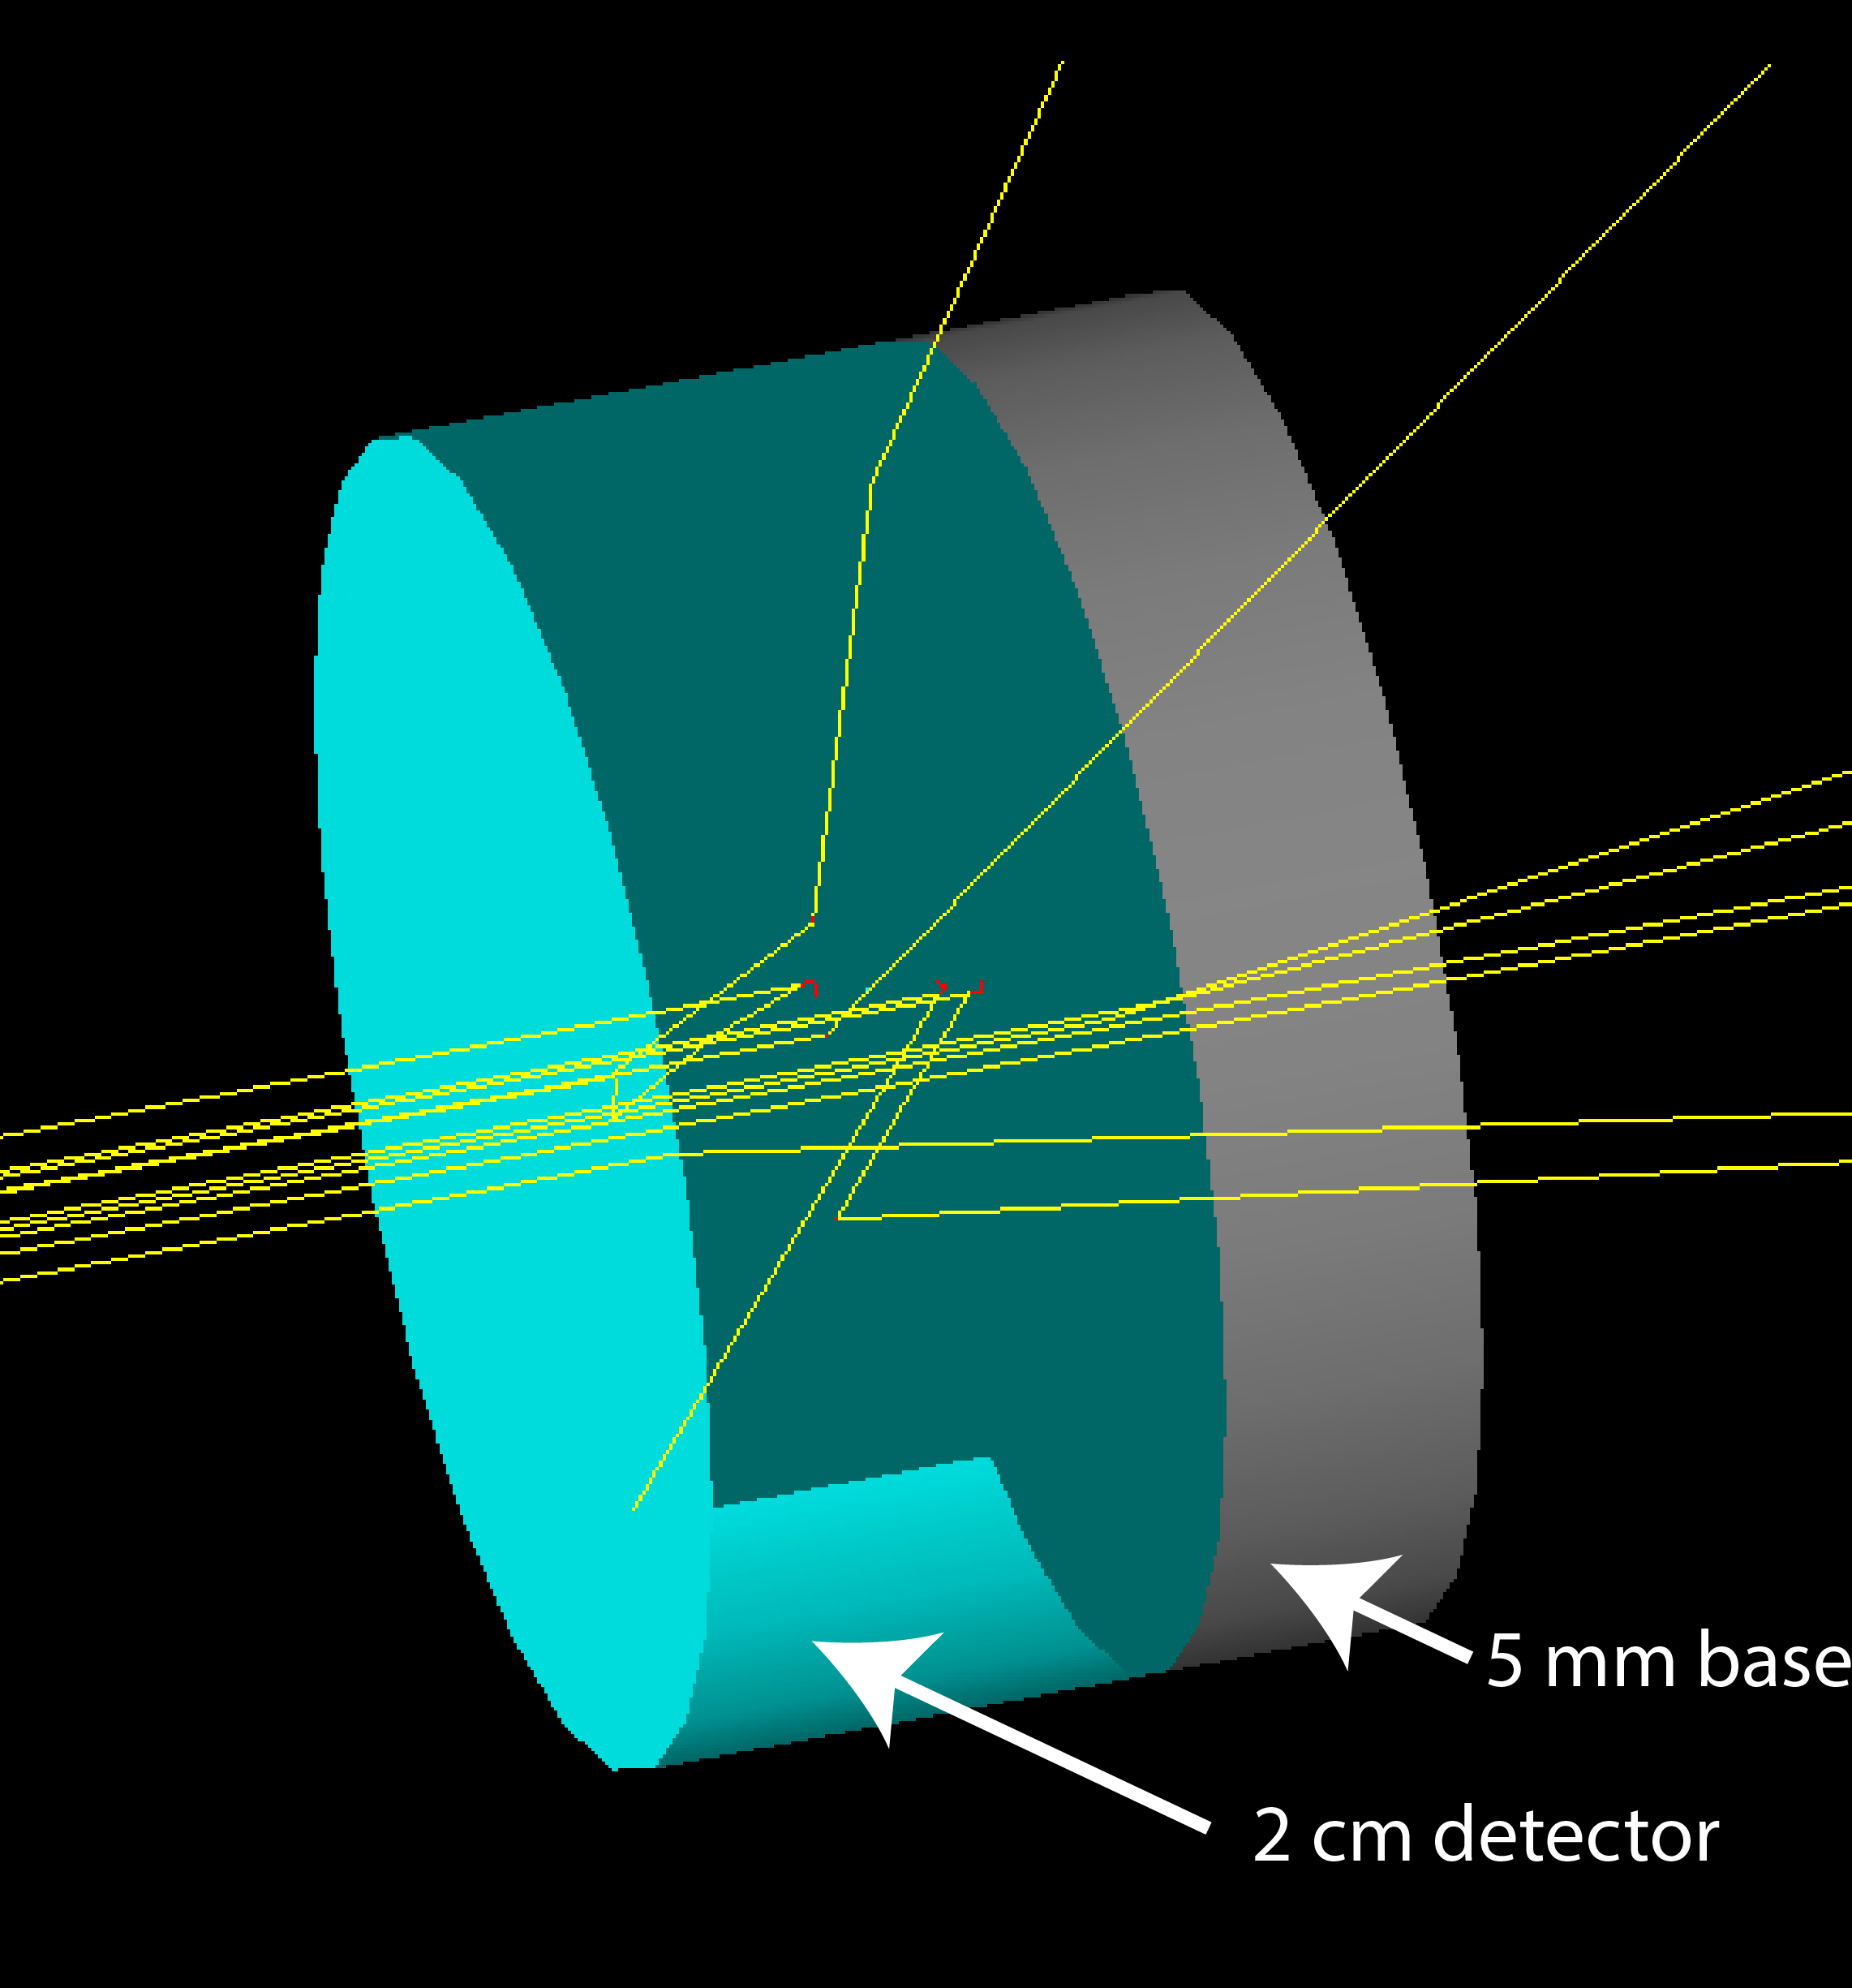
\includegraphics[width=\textwidth]{GEANT4AnnotatedGeo_EnergyDepEvent}
	\caption[GEANT4 Energy Deposition Geometry]{GEANT4 Geometry for the Simulation of Energy Deposition. What is shown are 10 photons from a \iso[60]{Co} source impingement upon a \SI{2}{\cm} thick detector.  The photon tracks are shown in yellow, while the electron tracks are shown in red.}
	\label{fig:EDepSimGeo}
\end{figure}
It is expected that the the Livermore data-driven parameterized electromagnetic physics will be necessary to calculate the ionizing energy deposition, extending the standard electro-magnetic physics down to \SI{1}{\kilo\eV}.
The neutron interactions will be simulated with a hadronic modules, using the \verb+HP+ flavored modules to use the ENDF cross sections to calculate the interaction rates.

\subsection{Simulation Validation}
The validation of this GEANT4 simulation was completed by reproducing the single collision energy loss in water as well as comparing  the spectral shapes and averages of simulated and measured spectra.
The reproduction of the single collision energy loss will ensure that the electron physics are implemented correctly, while the simulation of the polymeric film energy deposition allows the user to gain confidence that the correct tracking and binning analysis has been implemented.

\subsubsection{Single Collision Energy Loss}
The simulation was validated by reproducing the single collision energy loss for water as well as comparing spectra shapes and averages of simulated spectra to the measured spectra.
The single collision energy loss spectra for water that was simulated is shown in Figure \ref{fig:SingleCollisionELossWater}.
In general there was excellent agreement between the simulated energy spectra and a previously published spectra\cite{turner_comparative_1982}, with the simulated spectra having much better resolution than the reference did not.
It is thought that this is due to the water model in GEANT4 having better cross sections than the previously published spectra.
\begin{figure}[ht]
  \centering
  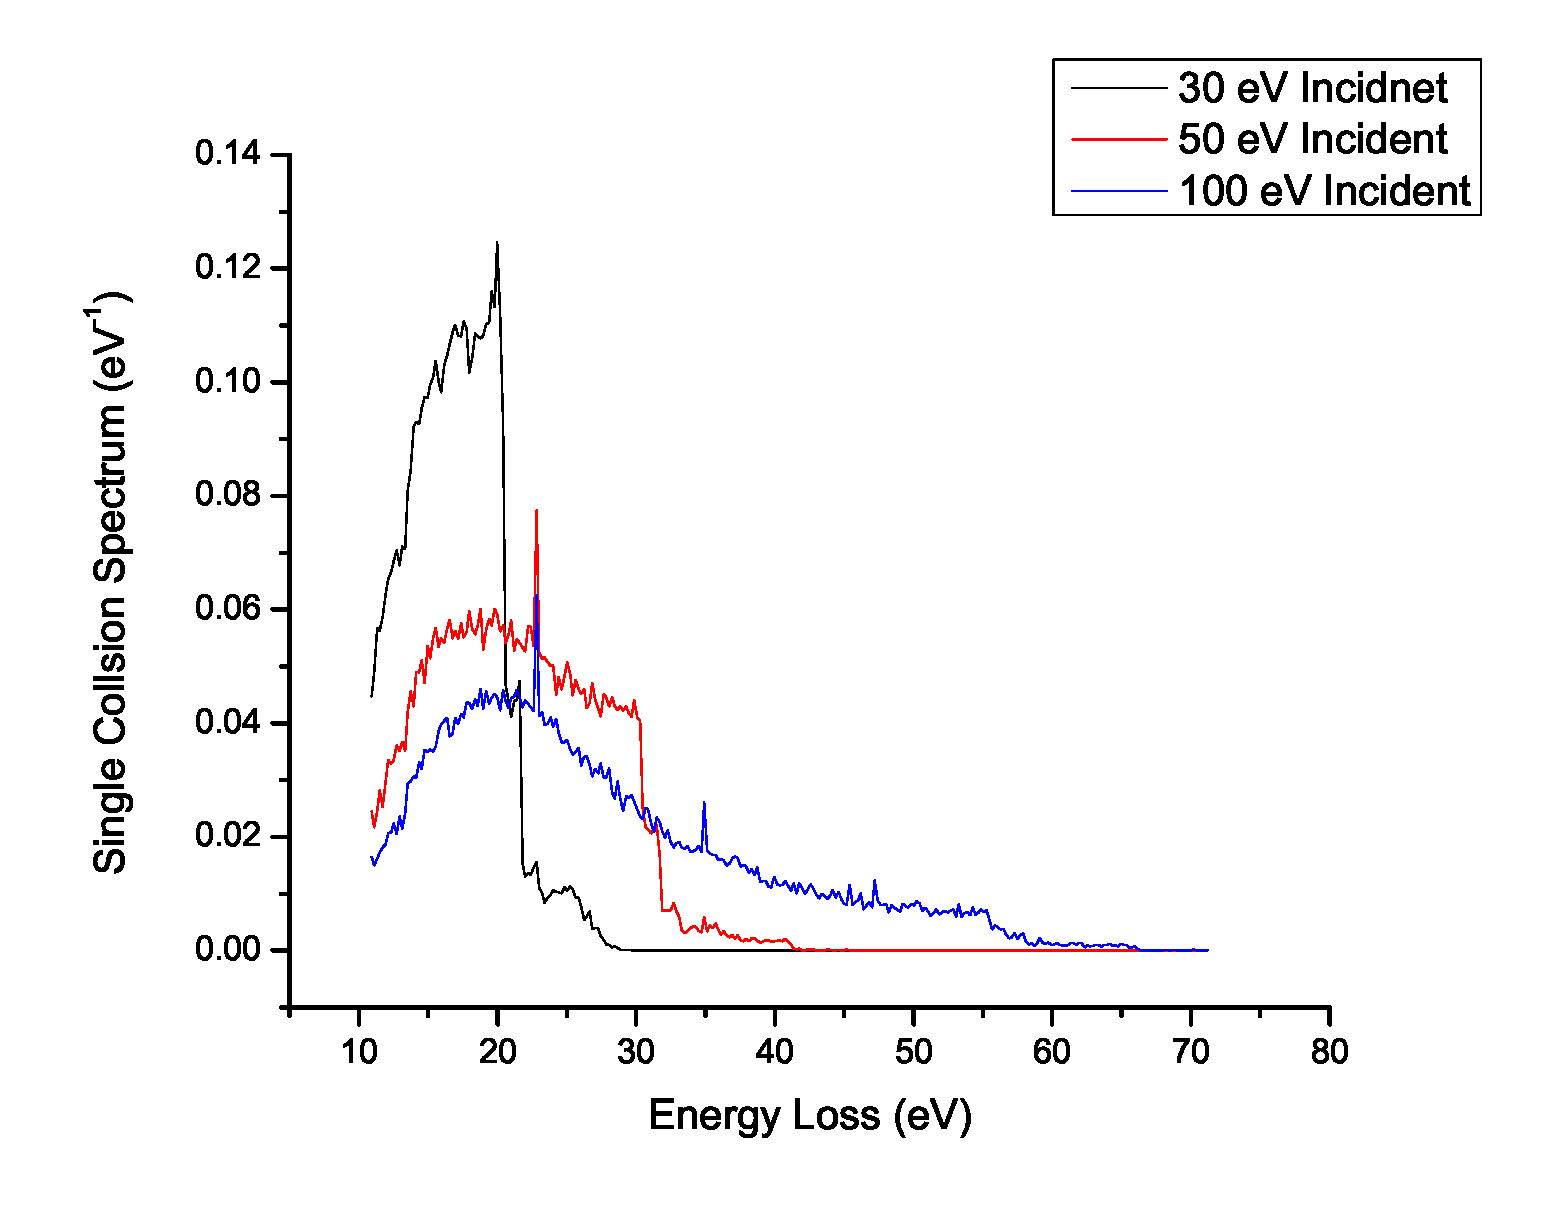
\includegraphics[width=\textwidth]{SingleCollisionEnergyLoss_300bins}
  \caption{Single Collision Energy Loss of Water. The simulated energy spectra matches that of Turner\cite{turner_comparative_1982}.}
	\label{fig:SingleCollisionELossWater}
\end{figure}

\subsubsection{Spectra Agreement}
The validity of the GEANT4 simulation is determined by comparing the spectra shapes of measured spectra to simulated energy deposition.
Figure \ref{fig:spectraComparisonGamma} shows the comparison between the simulated energy deposition per incident photon from a \iso[60]{Co} source and the measured pulse height spectra from the \iso[60]{Co} irridiator per incident photon.
The energy calibration on the upper axis of the measured spectra was completed by finding the channel number at a given intrinsic efficiency and the corresponding energy at that intrinsic efficiency.
The energy of this feature on the measured spectra was then compared to the energy on the simulated spectra, with all of the values being within 10\%.
\begin{figure*}[ht]
	\centering
	\begin{subfigure}[b]{0.45\textwidth}
    		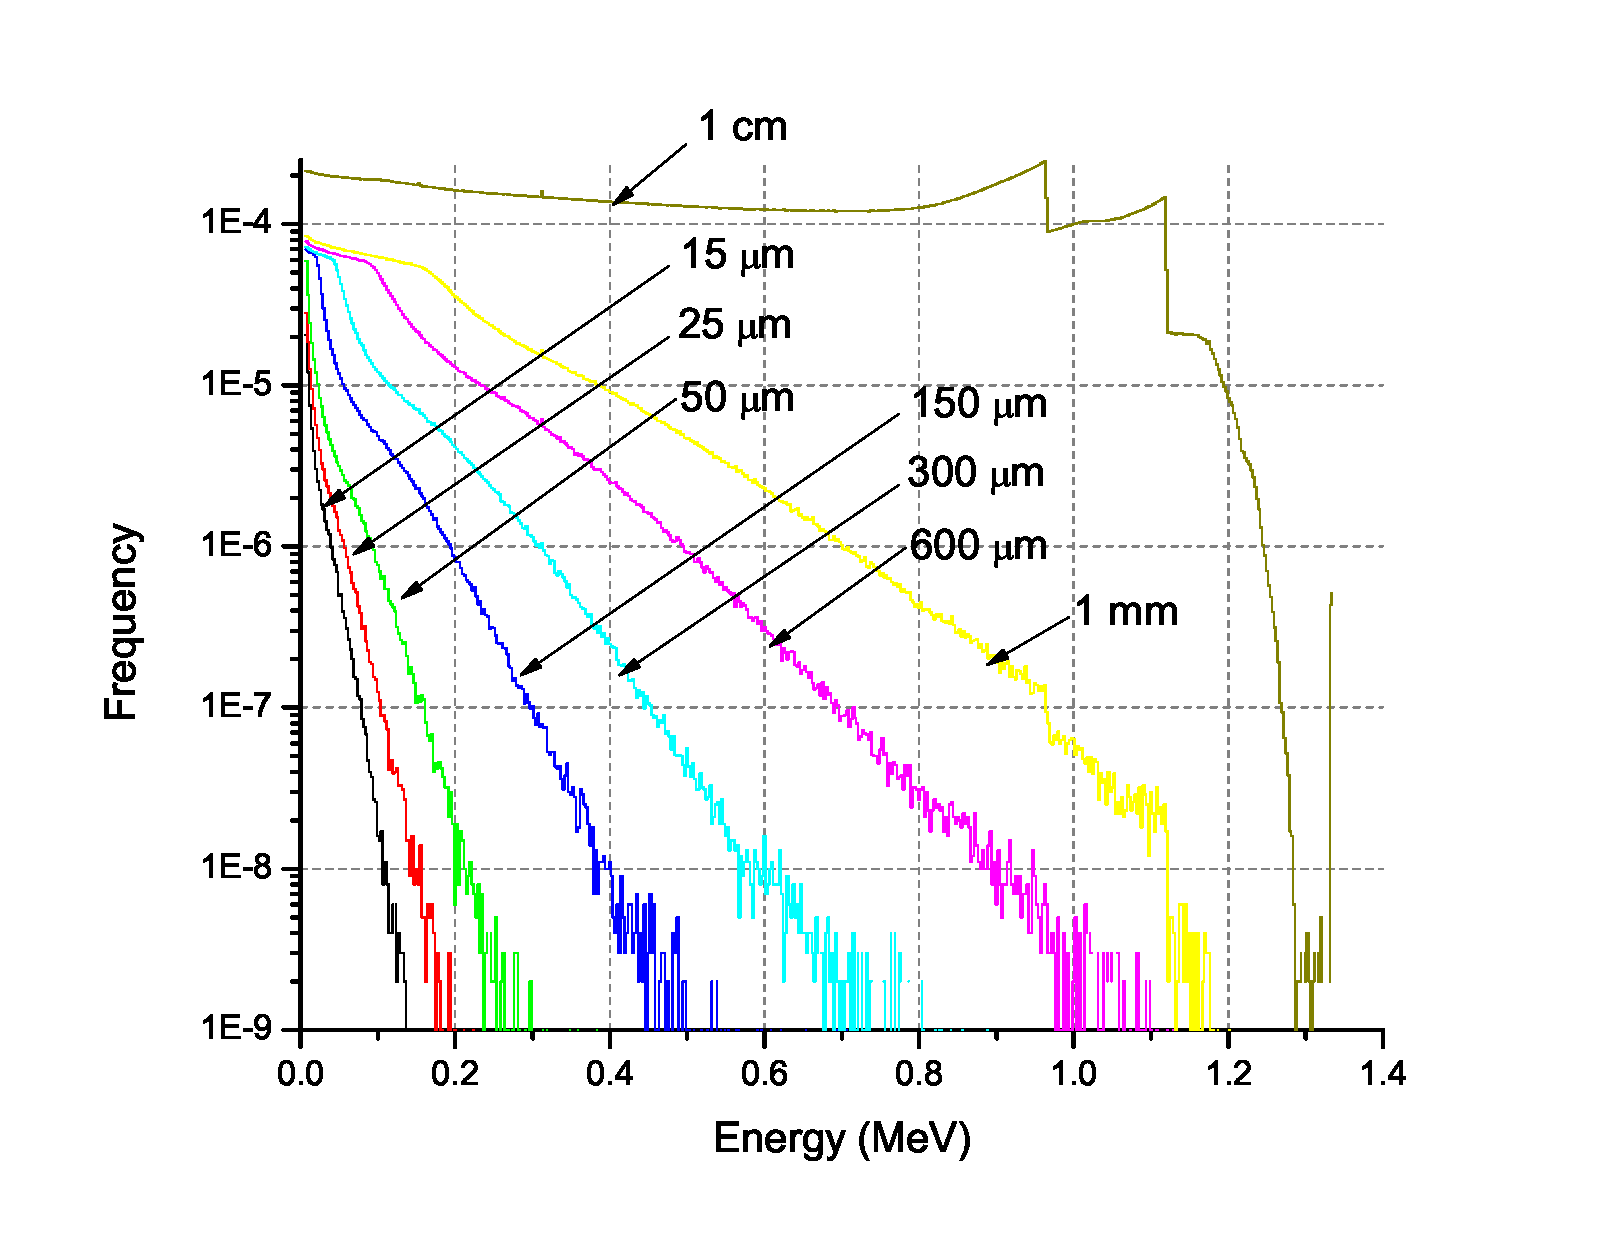
\includegraphics[width=\textwidth]{PS_EDepSim_Co60}
		\caption{GEANT4 Simulated Energy Deposition}
	\end{subfigure}%
	~
	\begin{subfigure}[b]{0.45\textwidth}
    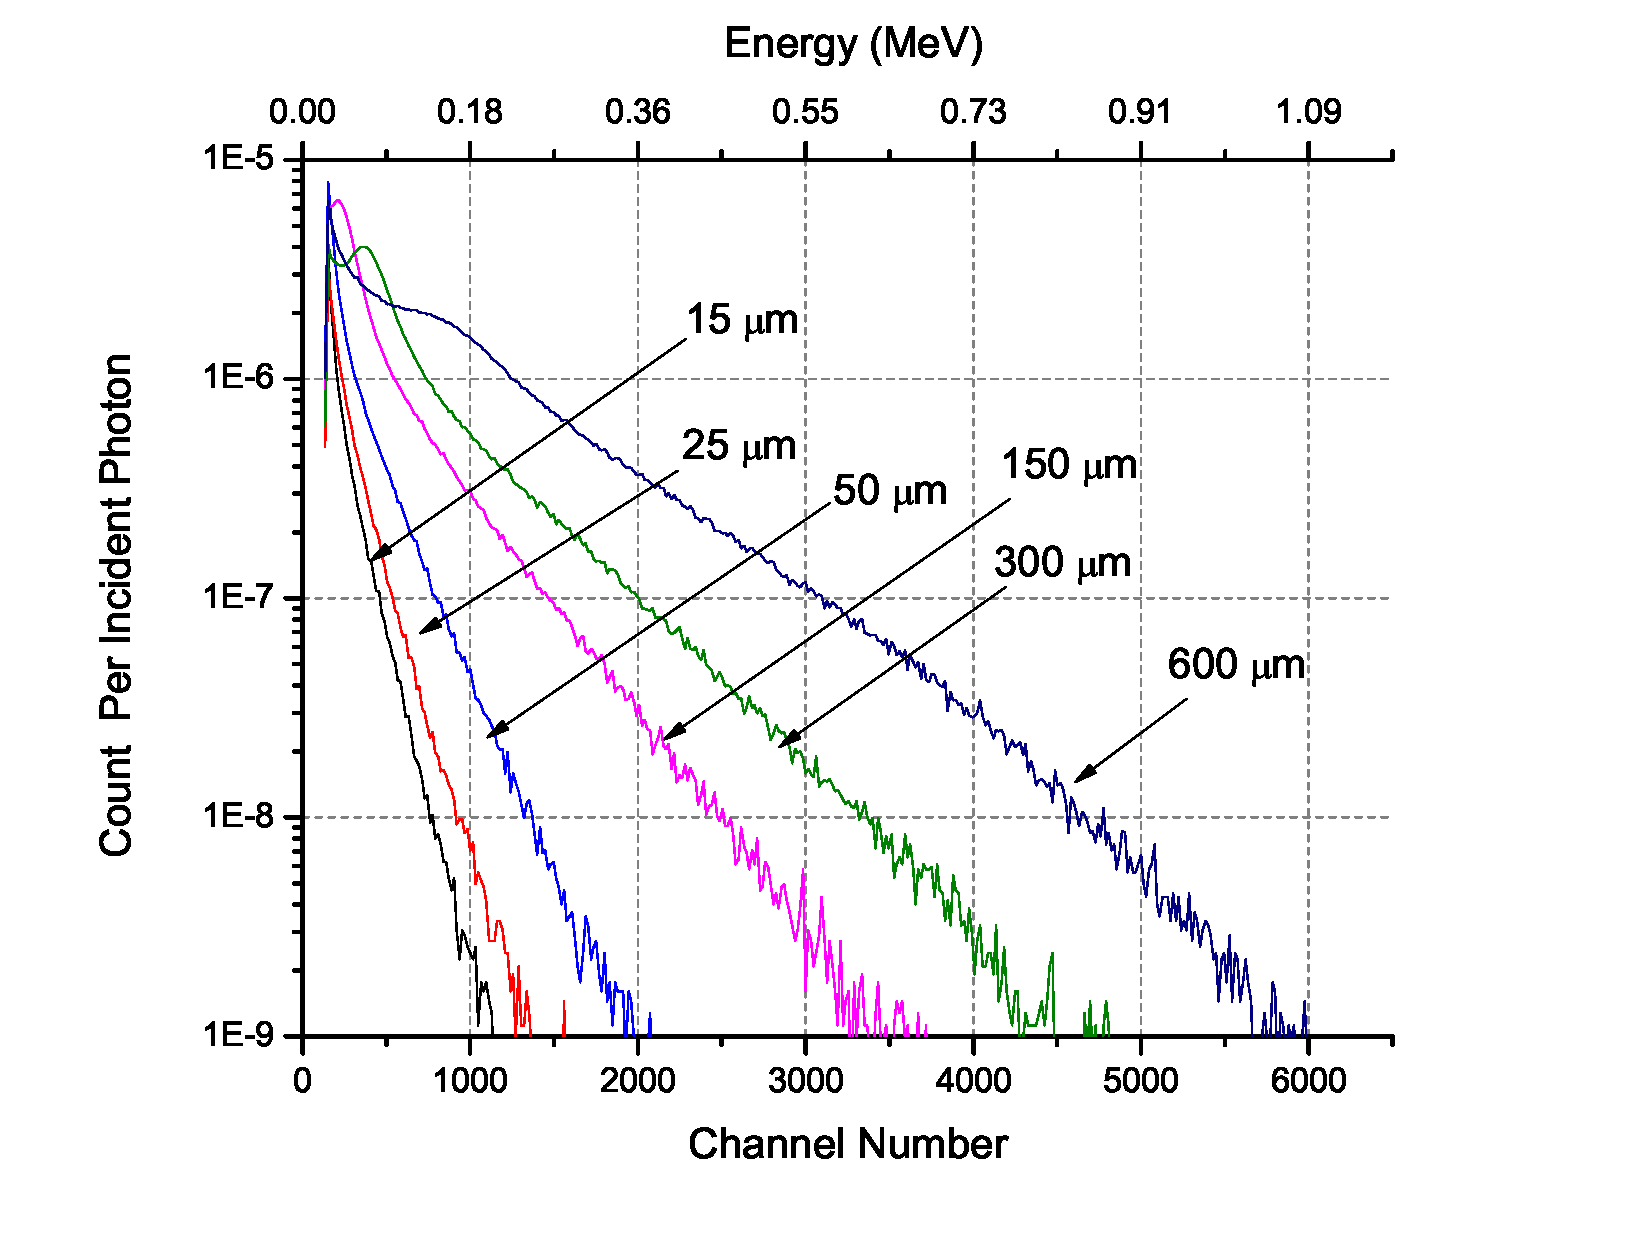
\includegraphics[width=\textwidth]{PS_GammaCR-Binned-FluxNorm_20LiF_5PPO}
		\caption{Measured Pulse Height Spectra}
	\end{subfigure}%
	\caption{Comparison of the energy deposition and binned pulse height spectra for validation. The spectra have the same shape, indicating agreement. The fabricated films greater than \SI{600}{\um} were of poor optical quality and therefore their results are not shown.}
	\label{fig:spectraComparisonGamma}
\end{figure*}
The average energy deposition and average pulse height are shown in Figure \ref{fig:EDepLightYield}. 
With the average energy deposition on the left axis and the average light yield (pulse height) on the right axis, it is possible to compare the measurement and the simulation and agreement is observed.
\begin{figure*}[ht]
	\centering
	\begin{subfigure}[b]{0.45\textwidth}
    		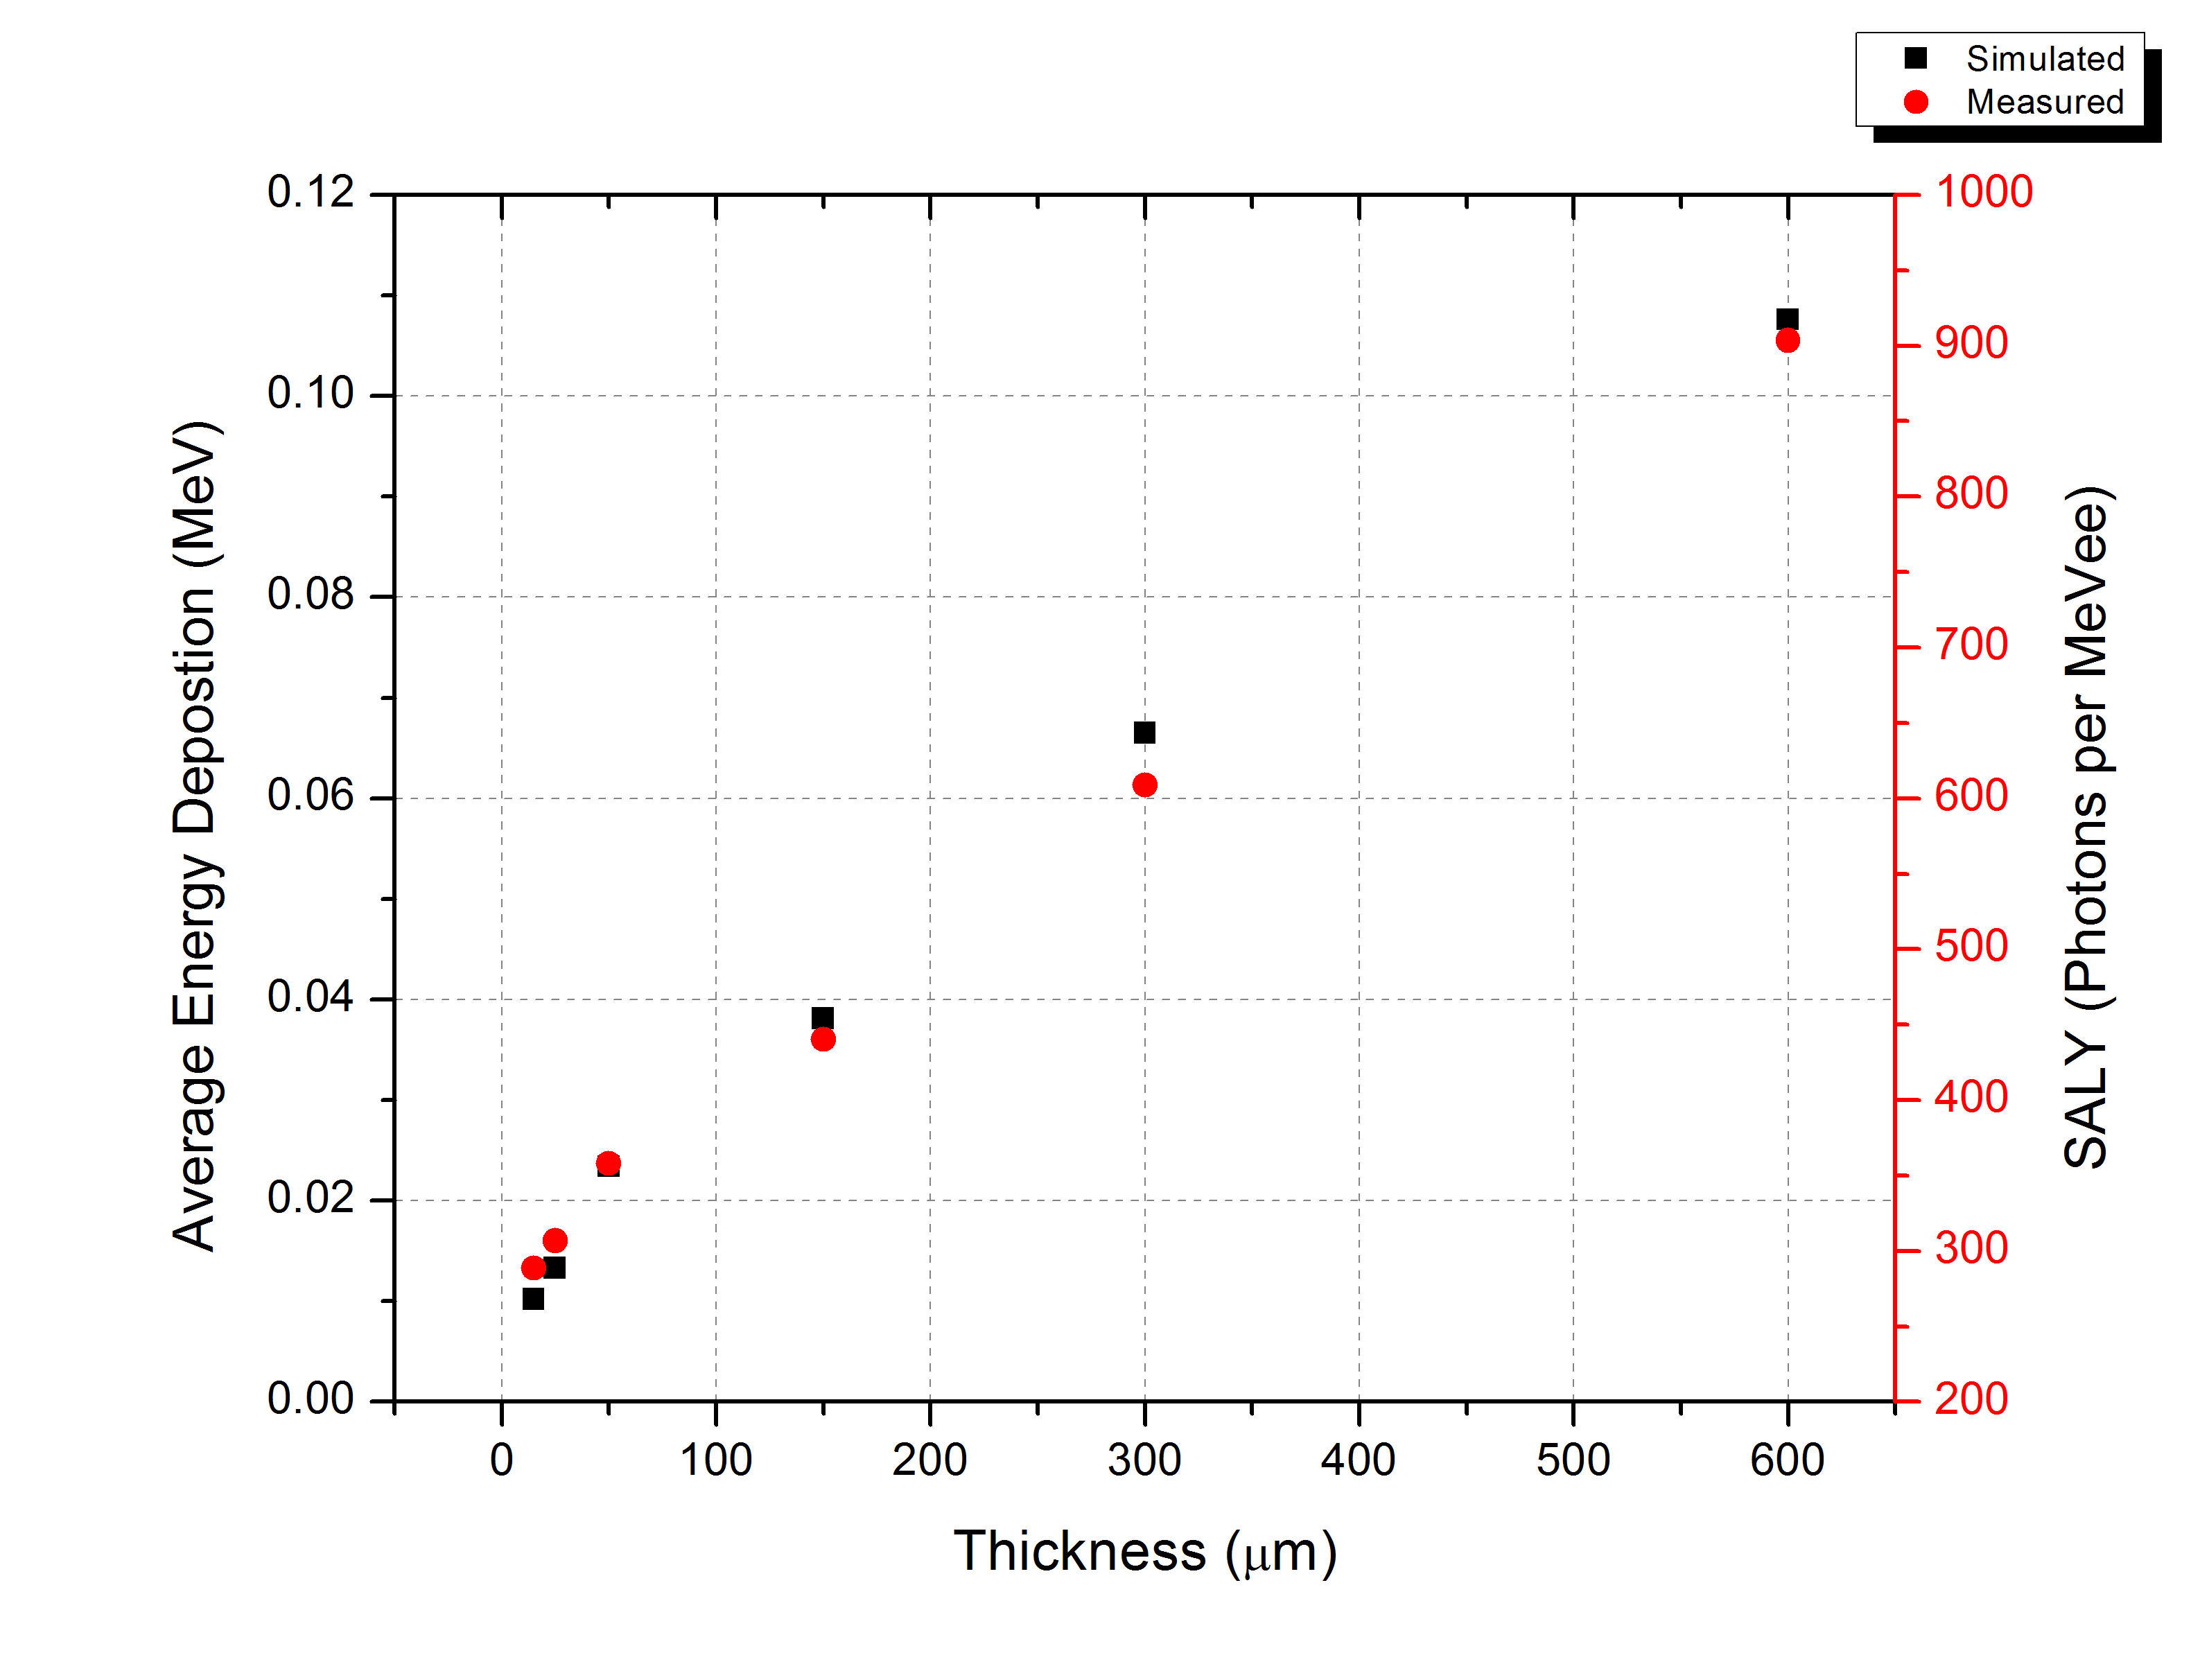
\includegraphics[width=\textwidth]{G4EDep_LightYield_Co60}
		\caption{Gamma (\iso[60]{Co})}
	\end{subfigure}%
	~
	\begin{subfigure}[b]{0.45\textwidth}
    		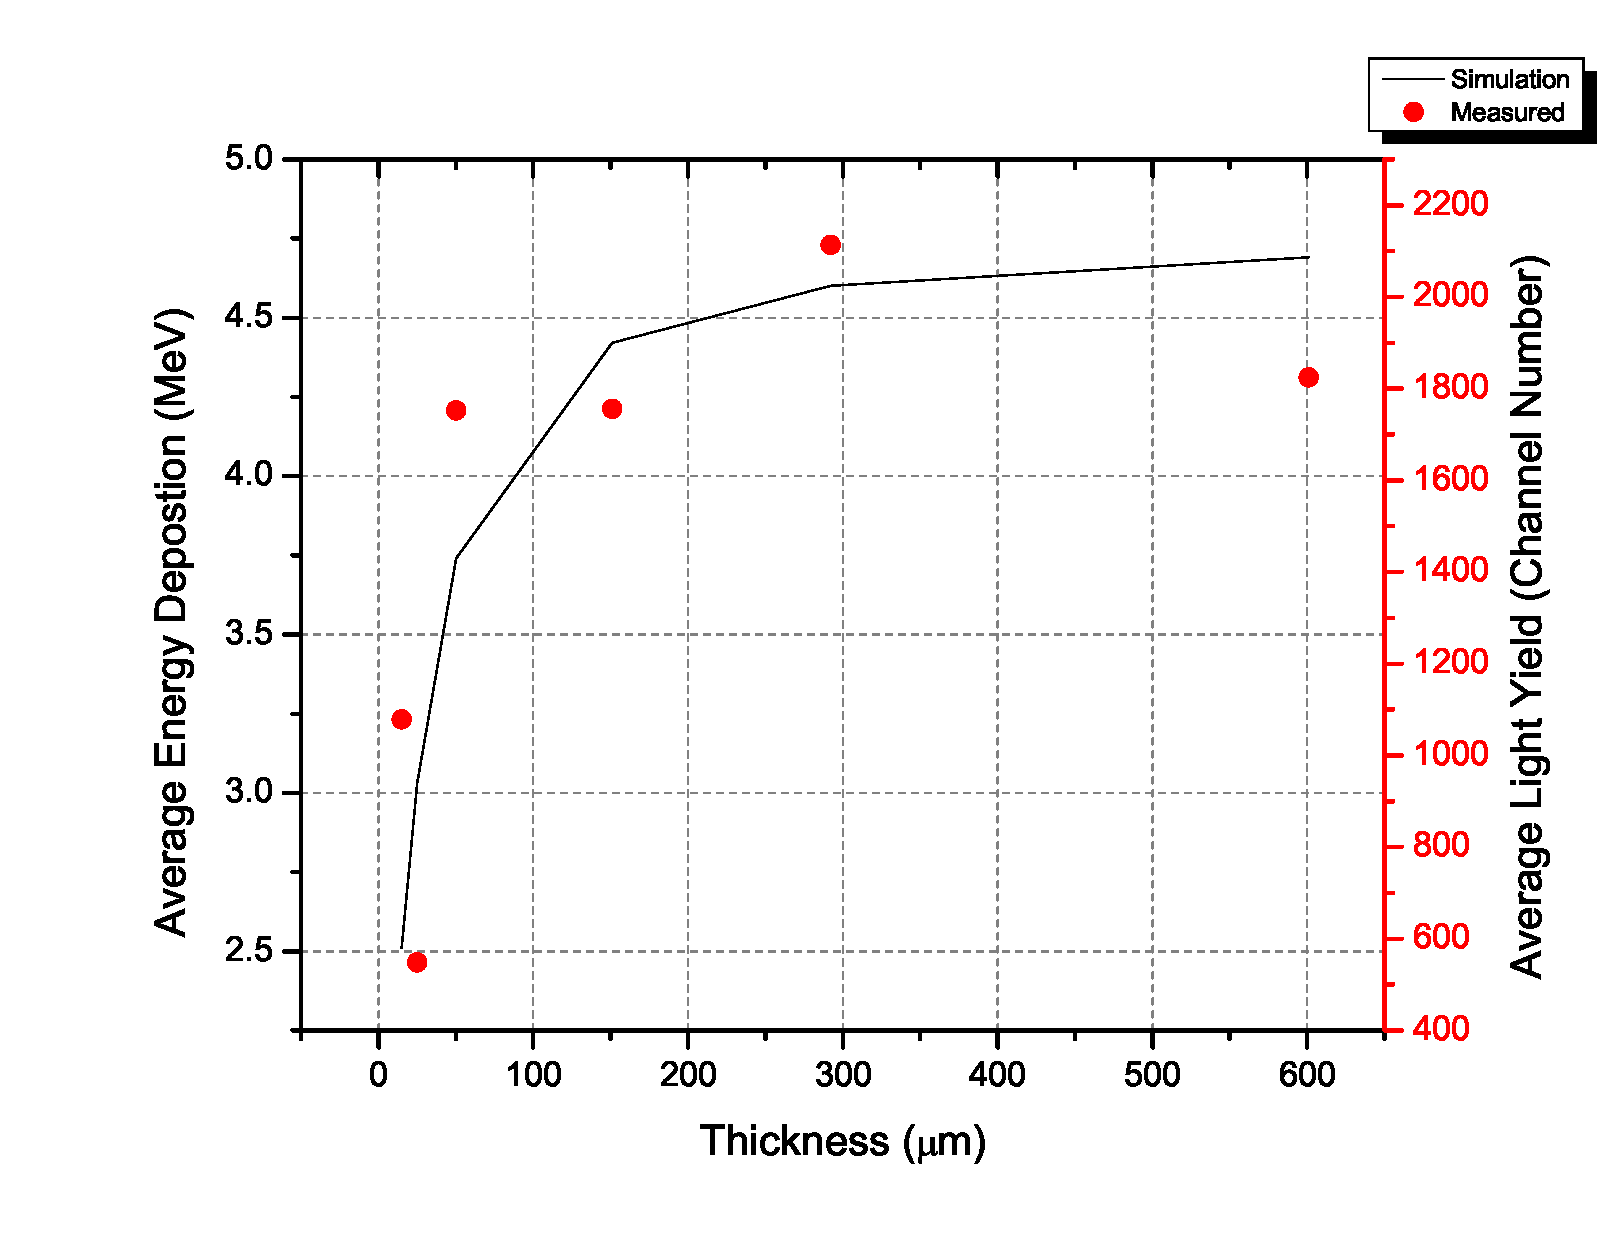
\includegraphics[width=\textwidth]{G4EDep_LightYield_Neutron}
		\caption{Neutrons}
	\end{subfigure}%
	\caption{Average Energy Deposition and Measured Light Yield. The solid lines are calculated values and the red dots are measurements.}
	\label{fig:EDepLightYield}
\end{figure*}


%%%%%%%%%%%%%%%%%%%%%%%%%%%%%%%%%%%%%%%%%%%%%%%%%%%%%%%%%%%%%%%%%%%%%%%%%%%
%                                                                         %
%                     RESULTS and ANALYSIS                                %
%                                                                         %
%%%%%%%%%%%%%%%%%%%%%%%%%%%%%%%%%%%%%%%%%%%%%%%%%%%%%%%%%%%%%%%%%%%%%%%%%%%
\section{Results}
\label{sec:Results}
The calculated gamma intrinsic efficiency for six polymeric films along with the neutron response of two of the films in Figure \ref{fig:GammaIntrNeutronCounts}, and the fraction of neutron counts above the MLLD necessary for a given gamma intrinsic efficiency is plotted in Figure \ref{fig:crVsIntEff}.
It is observed that if the films are thin enough (less than \SI{150}{\um}) it is possible to have a significant count rate above the mathematical lower level discriminator necessary for the pulse height discrimination of one in a million.
This is seen by the \SI{50}{\um} film and the \SI{150}{\um} film having the tail of their neutron spectra above the pulse height discriminator necessary for an intrinsic efficiency of \num{1E-6}.
Table \ref{tab:FractionCRGamma} shows the fraction of neutron count rate that is above the MLLD necessary for $\epsilon_{int,\gamma n} \le \si{1E-6}$.
Films less than \SI{50}{\um} have over 2\% of the counts above the necessary discriminator setting, while thicker films have have a factor of 10 less.
\begin{figure}[ht]
    \centering
    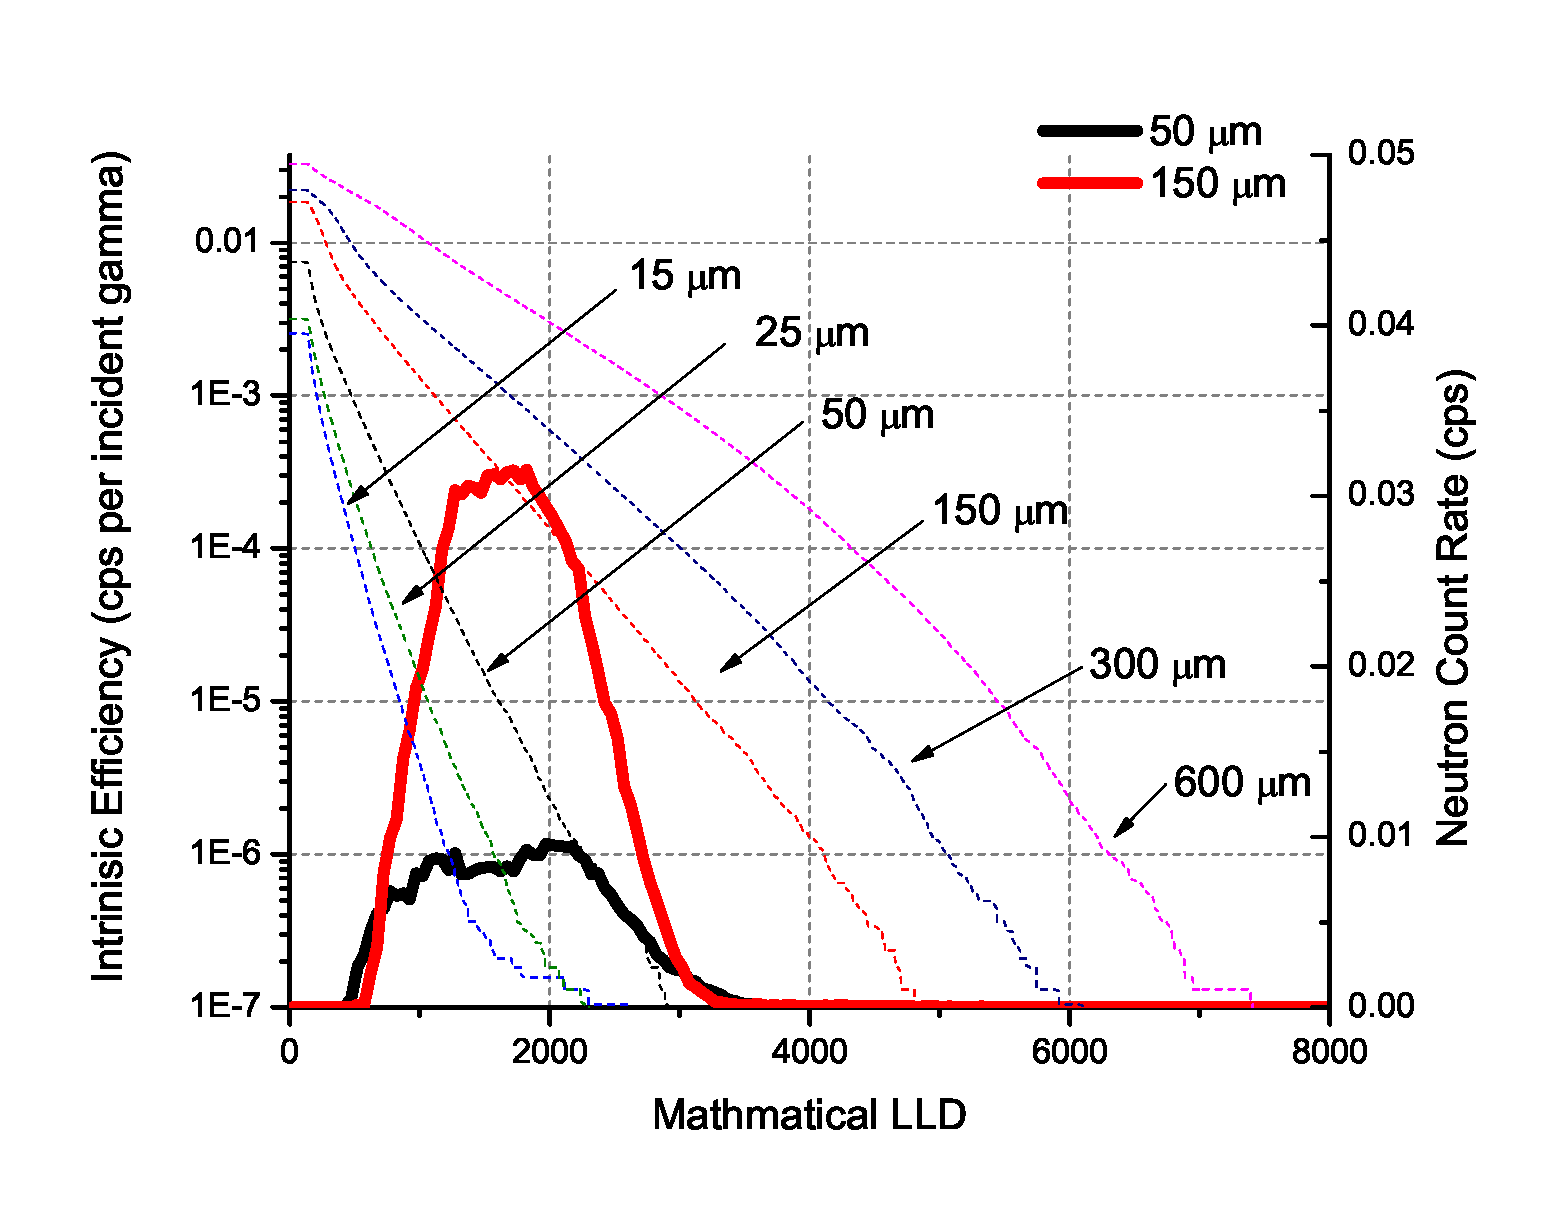
\includegraphics[width=\textwidth]{PS_IntEff_LiF20_PPO5}
    \caption[PS Gamma intrinsic efficiency and neutron count rate]{Gamma intrinsic efficiency (dashed lines) plotted against neutron counts (solid). The gamma spectra has been normalized by the number of incident photons upon the sample, while the neutron spectra has not.}
    \label{fig:GammaIntrNeutronCounts}
\end{figure}
\begin{figure}[ht]
    \centering
    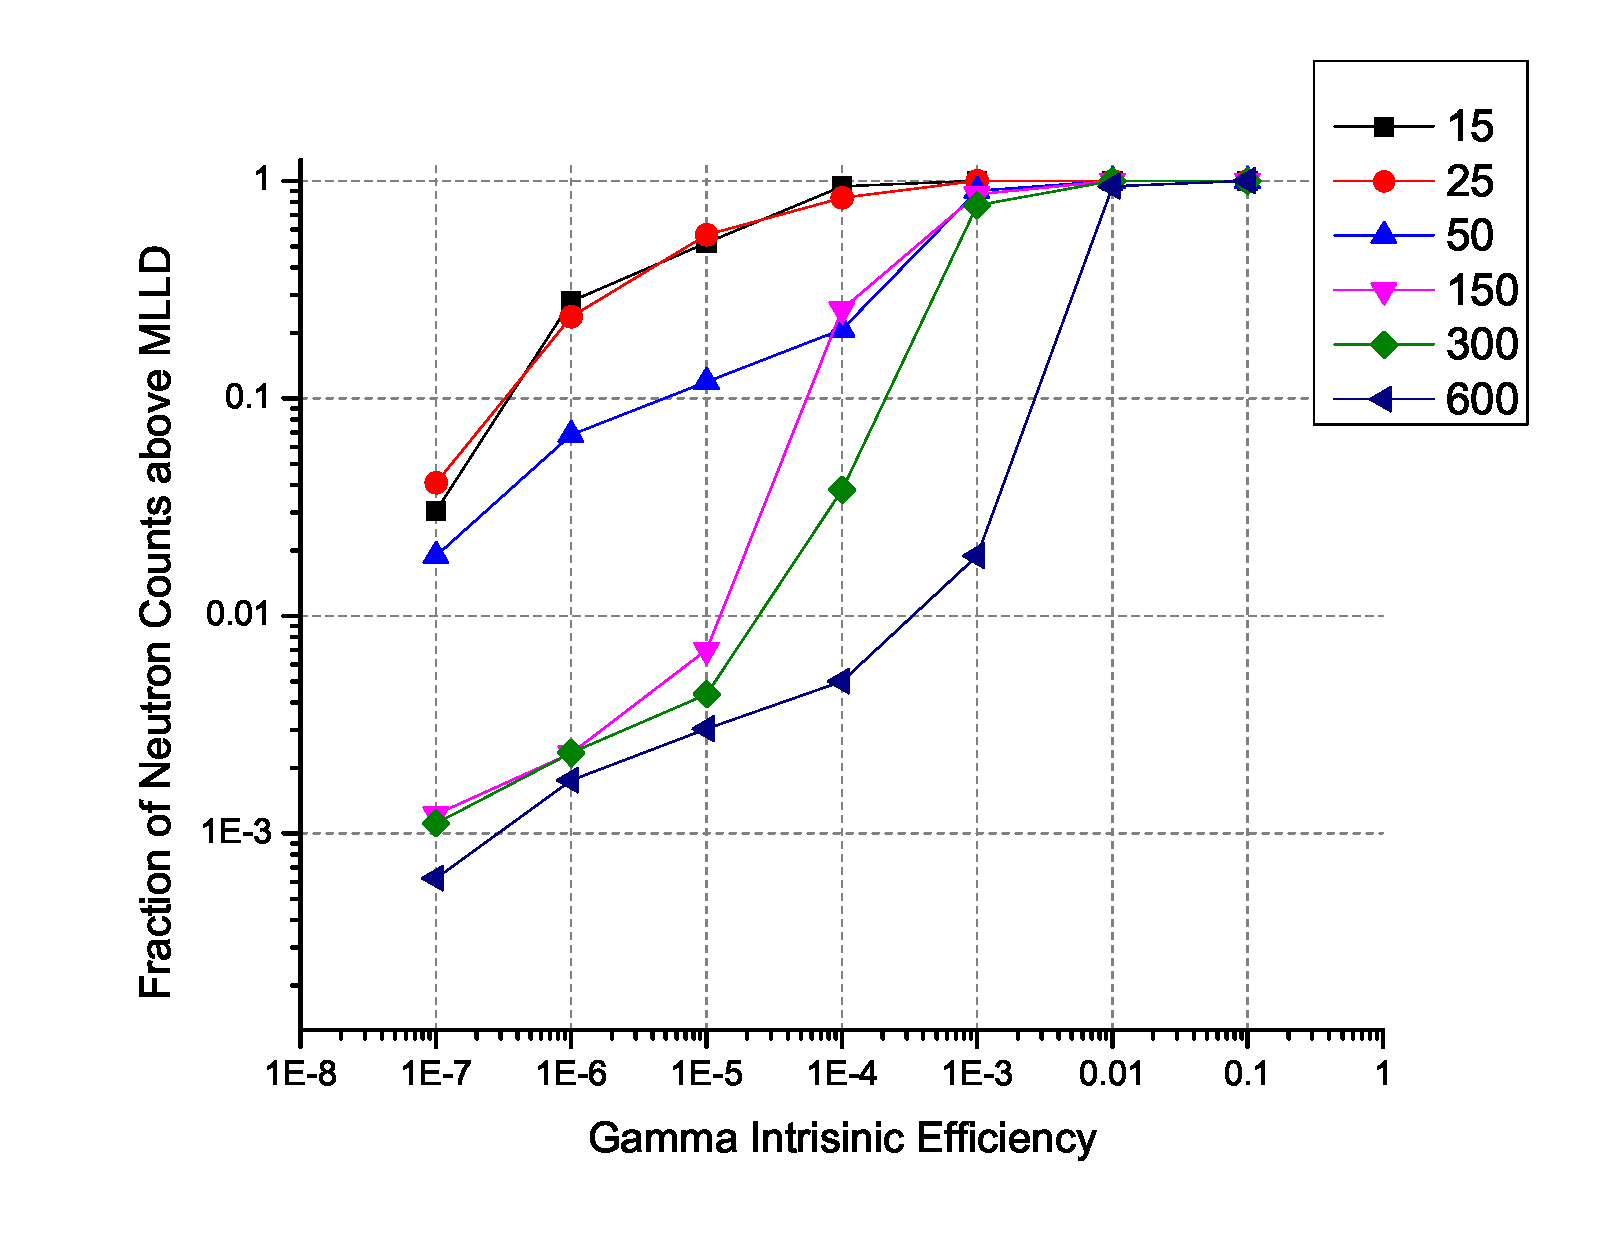
\includegraphics[width=\textwidth]{PS_IntFractionNCR_LiF}
    \caption{Intrinsic efficiency versus neutron count rate. }
    \label{fig:crVsIntEff}
\end{figure}
\begin{table}[]
    \caption{Fraction of Neutron Count Rate Above Discriminator Setting}
	\centering
	\begin{tabular}{c | c}
	Thickness & Neutron Fraction \\
	\hline
	\hline
	\SI{15}{\um} & 0.28 \\
	\SI{25}{\um} & 0.024 \\
	\SI{50}{\um}  & 0.067 \\
	\SI{150}{\um}  & 0.023 \\
	\SI{300}{\um}  & 0.023 \\
	\SI{600}{\um}  & 0.0017 \\
	\end{tabular}
  \label{tab:FractionCRGamma}
\end{table}
In addition it is observed in Figure \ref{fig:GammaIntrNeutronCounts} that for neutrons, thicker films only enhance the resolution of the film and do little to increase the light yield, as most of energy from a neutron event is captured in the film.
The average energy deposited was computed for each thickness and normalized by the incident energy for gammas by the Q-value of the reaction for neutrons, and is presented in Table ~\ref{tab:FractionEDep}.
For thickness greater than \SI{150}{\um} there is little benefit in increasing the thickness of the film in terms of energy deposition by neutrons, since over 90\% of the energy is being deposited in the film.
\begin{table}[ht]
    \caption{Fractional Energy Deposition for Various Thickness}
	\centering
	\begin{tabular}{c | c c}
	Thickness & Gamma Fraction & Neutron Fraction \\
	\hline
	\hline
	\SI{15}{\um} & 0.010 & 0.531 \\
	\SI{25}{\um} & 0.013 & 0.634 \\
	\SI{50}{\um} & 0.017 & 0.782 \\
	\SI{150}{\um} & 0.032 & 0.927 \\
	\SI{300}{\um} & 0.052 & 0.964 \\
	\SI{600}{\um} & 0.087 & 0.982 \\
	\SI{1}{\mm} & 0.130 & 0.989 \\
	\SI{1}{\cm} & 0.425 & 0.998 \\
	\end{tabular}
  \label{tab:FractionEDep}
\end{table}

Figure \ref{fig:simKinE} illustrates the simulated kinetic energy of secondary electrons from Compton scattering and from alpha and triton interactions.
It is observed that kinetic energy of the secondary electrons from the neutron reaction products have predominately energies in the kilo-volt range, while the Compton scattering electrons have energies in hundreds of kilo-volts range. 
However, it should be noted that there is only one secondary electron from a Compton scattering and multiple secondary electrons from the reaction products.
Figure \ref{fig:ReacProdDist} shows the distribution of the number of secondary electrons from the alpha and triton and their kinetic energy.
\begin{figure}[ht]
    \centering
    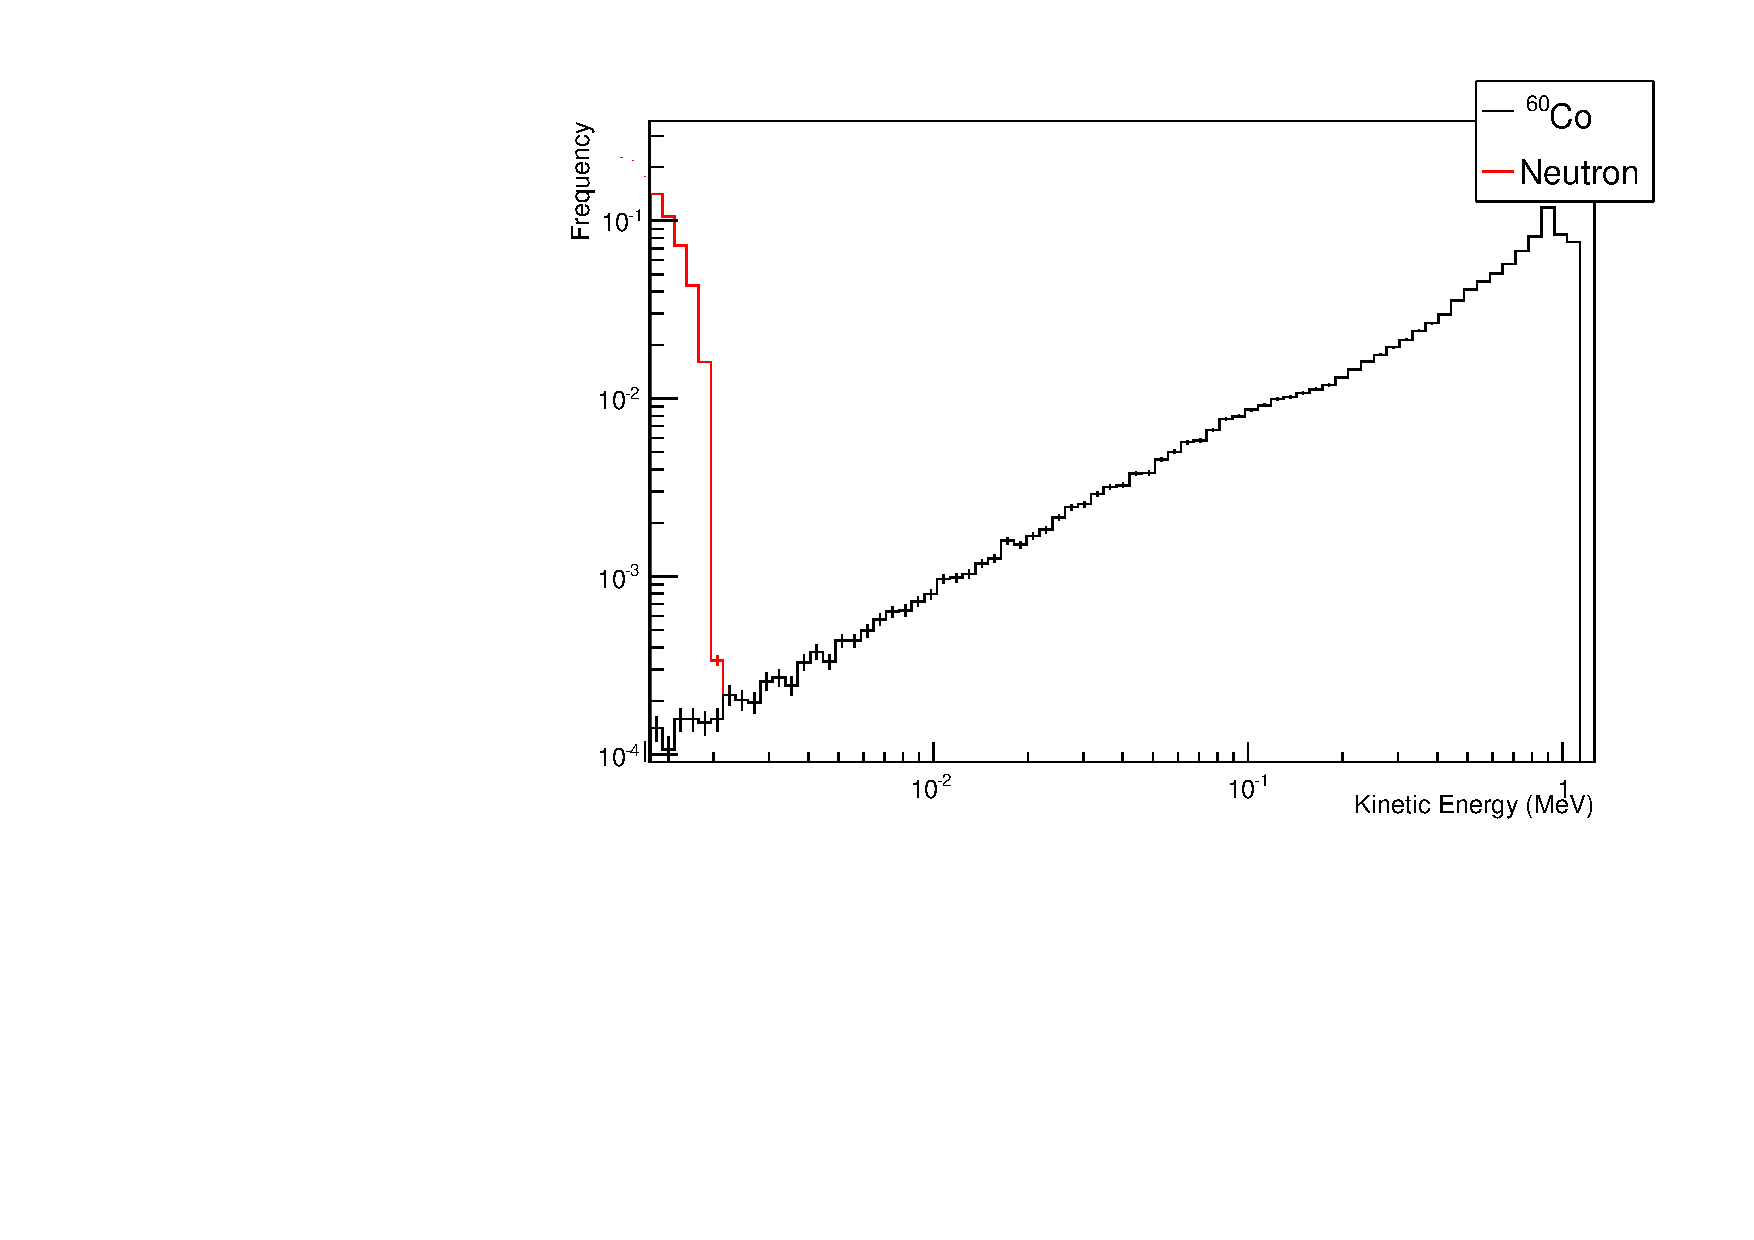
\includegraphics[width=\textwidth]{NGSecElecKinEDist}
    \caption{Simulated Kinetic Energy of Secondary Electrons from Compton Scattering and from \iso[6]{Li} reaction products}
    \label{fig:simKinE}
\end{figure}
\begin{figure*}[ht]
	\centering
	\begin{subfigure}[b]{0.45\textwidth}
    		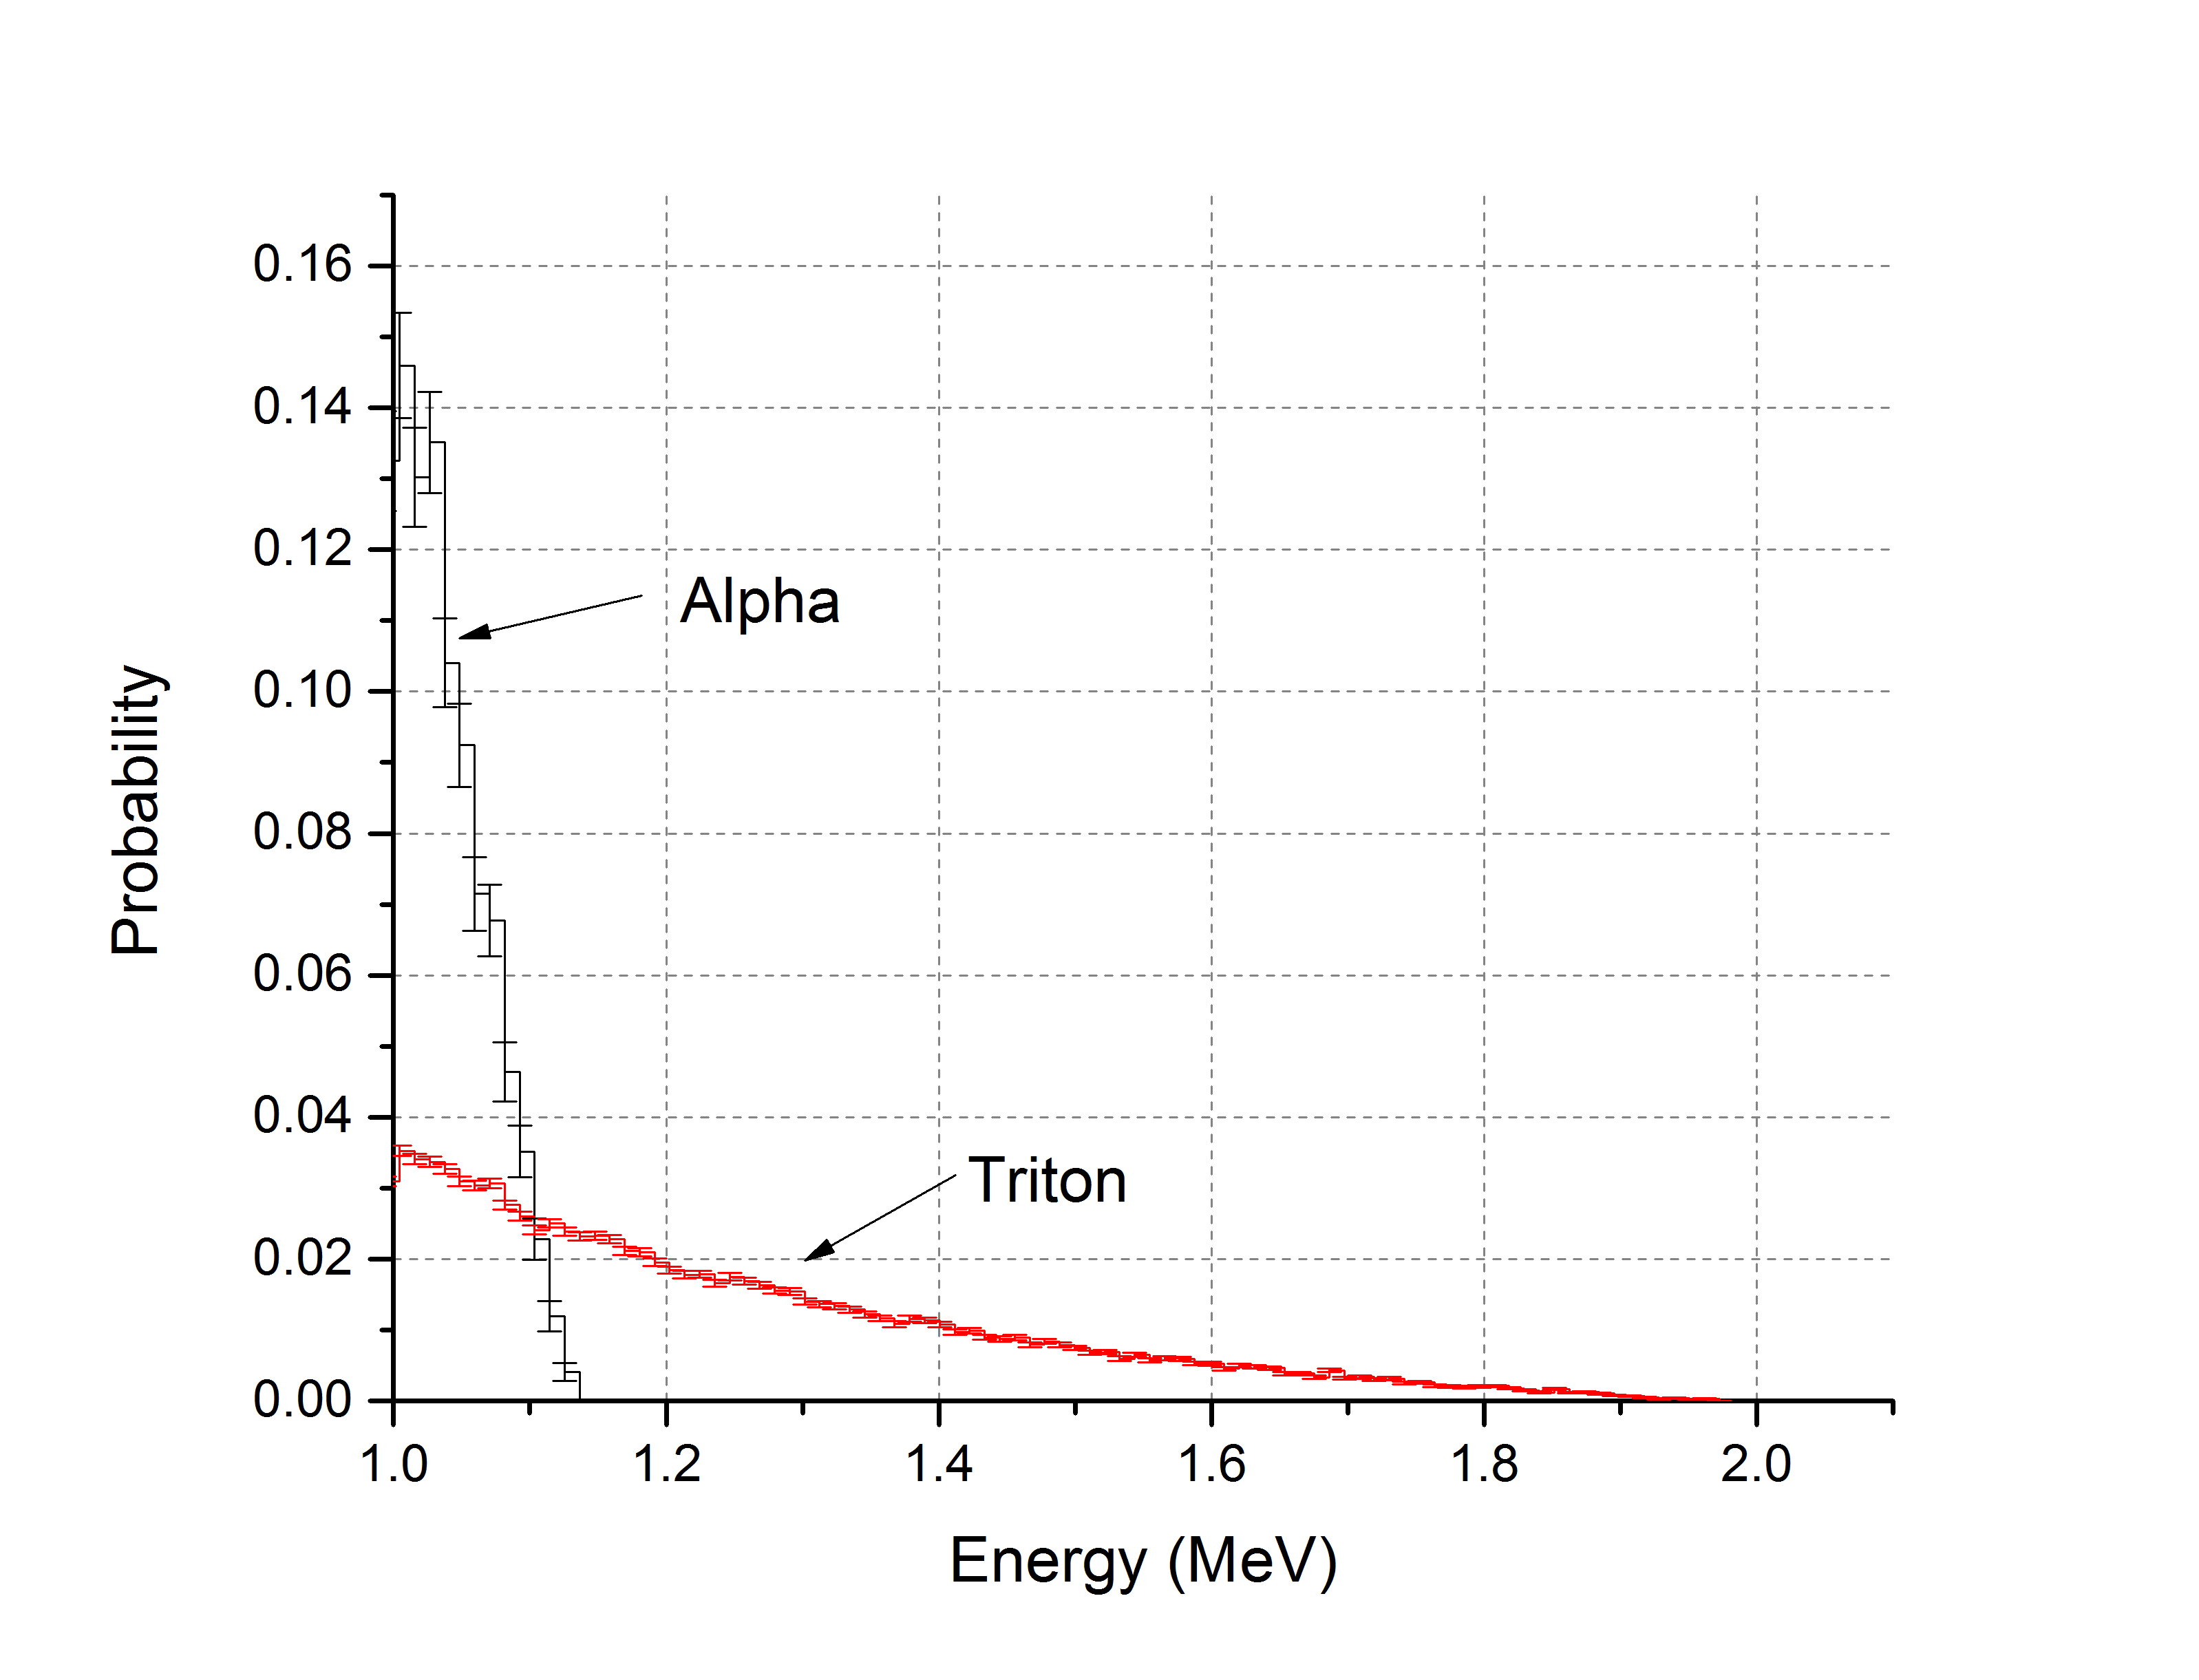
\includegraphics[width=\textwidth]{AlphaTritonSecElecKinEDist}
		\caption{Alpha and Triton Secondary Electron Kinetic Energy Distribution}
	\end{subfigure}%
	~
	\begin{subfigure}[b]{0.45\textwidth}
    		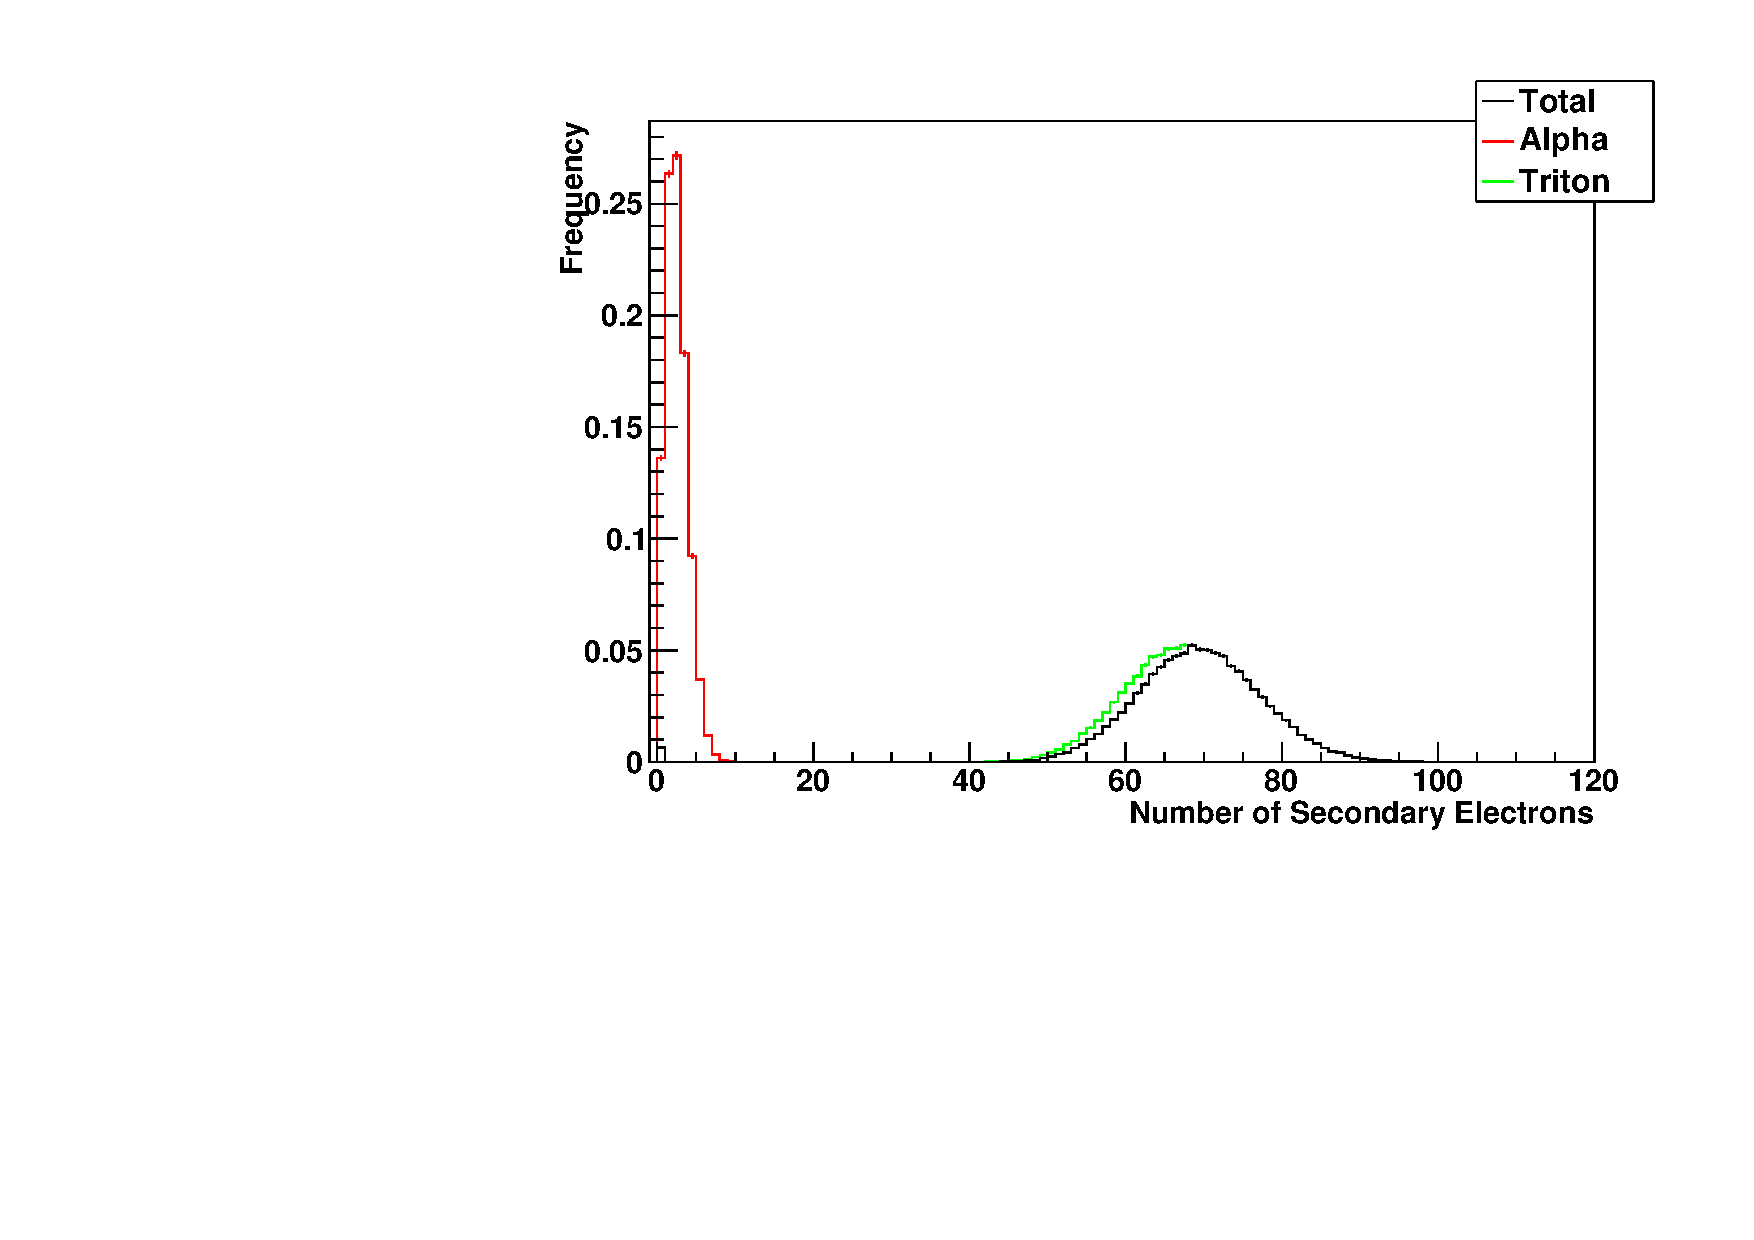
\includegraphics[width=\textwidth]{NeutronNumSecElec}
		\caption{Number of Secondary Electrons Produced Per Neutron Interaction}
	\end{subfigure}%
	\caption{Neutron Reaction Products Secondary Electrons Energies}
	\label{fig:ReacProdDist}
\end{figure*}
